\documentclass[10pt,xcolor=x11names,compress, show notes]{beamer}% pour l'impression, tout n'apparait qu'une fois \documentclass[handout,12pt]{beamer}

%\usepackage[scaled]{helvet}
\usepackage[round]{natbib}
\usepackage[utf8x]{inputenc}
\usepackage[USenglish]{babel}
\usepackage{todonotes}
\usepackage{color}
\usepackage{pbox}
\usepackage{graphicx}


\usepackage{changepage}
\usepackage{pifont} %pour les symbole sympa \ding{nb}

\usepackage{subfig}

%%% Pour Tikz
\usepackage{tikz}
\usetikzlibrary{calc}
\usetikzlibrary{shapes}
%\usetikzlibrary{arrows,shapes,trees,positioning}  

%%%pour les plots matlab en tikz
\usepackage{pgfplots} 
\pgfplotsset{compat=newest}

%%% Pour les maths
\usepackage{bm}
\usepackage{amsmath,mathtools}
\usefonttheme[onlymath]{serif}
\usepackage{cancel} %pour barrer des math

%%% Pour la mise en forme
\usepackage[export]{adjustbox}
%\usepackage{subcaption}
\usepackage{wrapfig}
\usepackage{pdfpages}
\setbeamertemplate{navigation symbols}{} 
\usepackage{array}
%\usepackage{subfigure}
%\usepackage[]{geometry}
%\usepackage{palatino}
%\setbeamertemplate{caption}{\raggedright\insertcaption\par}
\usepackage{multicol}
\setlength{\columnsep}{0cm}
\usepackage[framemethod=TikZ]{mdframed}

%%% Theme
\def \pied {~~~A. Dinsenmeyer~|~\insertshorttitle \hfill \insertframenumber/\inserttotalframenumber~~~} %content if footline
\usetheme{Alice}

%personnalisation
\definecolor{green}{rgb}{0,0.5,0} 

%figure csm
\newlength{\pas}	\setlength{\pas}{0.2cm}
\newcommand{\nbpas}{7}

%\setbeamertemplate{footline}{test}


%\useoutertheme[subsection=false]{miniframes} %%pour avoir le défilement en en-tête des diapos par section
%\setbeamercolor*{lower separation line head}{bg=DeepSkyBlue4} 

% Customisation 
\setlength{\fboxrule}{0.2pt}
\newcommand{\tikzmark}[1]{\tikz[remember picture] \coordinate (#1) ++ (-3pt,6pt) {};}
\newcommand{\citeTransp}[1]{\color{fg!50} \citep{#1}}
\renewcommand\bibsection{\section[]{~}}
\usepackage{algorithm}
\usepackage{algorithmic}
\graphicspath{{images/}}

%% Autre

\definecolor{main}{rgb}{0,0.407843137,0.545098039}%{0 0.439  0.753} %bleu %0 112 192
\definecolor{rouge}{rgb}{1 0.270 0 } %255 69 0
\definecolor{jaune}{rgb}{1 0.745 0} %255 190 0
\definecolor{vert}{rgb}{0.573 0.792 0.209} %146 202 74
\definecolor{source}{rgb}{0,0.5,0} 

\newlength{\avion}
\setlength{\avion}{0.6\textwidth}

\newlength{\larg}	\setlength{\larg}{0.5cm}	
\newlength{\haut}	\setlength{\haut}{4\larg}

\newcommand{\diag}[1]{\lceil#1\rfloor}
\newcommand*\circled[1]{\tikz[baseline=(char.base)]{
            \node[shape=circle,draw,inner sep=2pt,color=main,fill=main!10, line width=1pt] (char) {#1};}}

%%% Page de titre
%======================
\author{\underline{A. {Dinsenmeyer}}$^{1,2}$, Q. {Leclère}$^1$, J. {Antoni}$^1$ et E. Julliard$^3$}
\institute{$^1$ Laboratoire Vibrations Acoustique\\ $^2$ Laboratoire de Mécanique des Fluides et d’Acoustique\\Lyon, France \\ $^3$ Airbus, Toulouse}
\title{Débruitage de la matrice interspectrale pour l'étude des sources aéroacoustiques}
\subtitle{}
\titlegraphic{ 
\includegraphics[height=1cm]{logo/LABEX_CELYA.jpg} \hfill
 	  
\includegraphics[trim={0 3cm 0 3cm},clip=true,height=1cm]{logo/logo_ADAPT.png} \hfill
 
\includegraphics[height=1cm]{logo/LVA_compact_couleur.jpg} \hfill
 
\includegraphics[height=1cm]{logo/logo_lmfa.pdf} \hfill  }
\date{\small \vfill Journée CeLyA -- Mars 2019}
\begin{document}

%%%		Title
%======================
\begin{frame}[plain,t]
	\maketitle	
\end{frame}

%%% Context
%======================
\section*{Contexte}
\begin{frame}[t]{\insertsectionhead}
\vspace{0.2cm}
\begin{overlayarea}{\textwidth}{0.3\textheight}
\only<1-3>{
	\noindent\begin{minipage}{1.1\textwidth}
		\begin{itemize}
		        \item<1-> \textbf{Mesures bruitées} : Extérieur venté, soufflerie, milieu sous-marin, etc.
		        	\item<2-> \textbf{Contexte industriel} : design moteur et profil			
		        \item<3-> 2 types de fluctuations de pression : \\
			$ \left. \begin{array}{l} 
			\mbox{- les sources acoustiques (\textcolor{source}{signal})} \\                   
			\mbox{- la turbulence de l'écoulement (\textcolor{rouge}{bruit})}                      
			\end{array} \right\} \mbox{~SNR très faible voire négatif}$ 
		\end{itemize}
\end{minipage}
}
\end{overlayarea}
\vfill
\begin{minipage}{\textwidth}
		\centering
		\includegraphics<2>[width=\avion]{avion2.eps}
		%\includegraphics<2>[width=\avion]{avion2.eps}
		%\includegraphics<+>[width=\avion]{avion3.eps}
		%\includegraphics<3>[width=\avion]{avion4.eps}
		\includegraphics<3->[width=\avion]{avion5.eps}
	\end{minipage}
	
\end{frame}

\begin{frame}[t]{\insertsectionhead}
	\begin{center}
		\textcolor{black}{\bfseries \centering  Comment séparer la contribution des sources acoustiques et le bruit de couche limite turbulente ?}
	\end{center}
	\vfill

{ \bfseries Les méthodes existantes }
	\begin{itemize}
        		\item méthodes expérimentales : mousse, kevlar, microphones déportés,...
        		\item soustraction du bruit de fond
        		\item filtrage en nombres d'onde
        		\item si les mesures sont suffisamment longues : post-traitement (ex : problème inverse)
	\end{itemize}

	\vfill
\onslide<2->{
{\bfseries Méthodes proposées}
	\begin{itemize}
		\item Résolution d'un problème inverse : retrouver la contribution des sources
		\item Utilisation de signaux de référence non-bruités
	\end{itemize}
}
\end{frame}

\begin{frame}{Plan de la présentation}
	\tableofcontents[]
\end{frame}

\section{La matrice interspectrale}
\begin{frame}{\insertsectionhead}
	\centering
	\small Spectres moyennés (processus stationnaire)\\[1em]
	\begin{tikzpicture}	
		\node (mic) at (0,0) {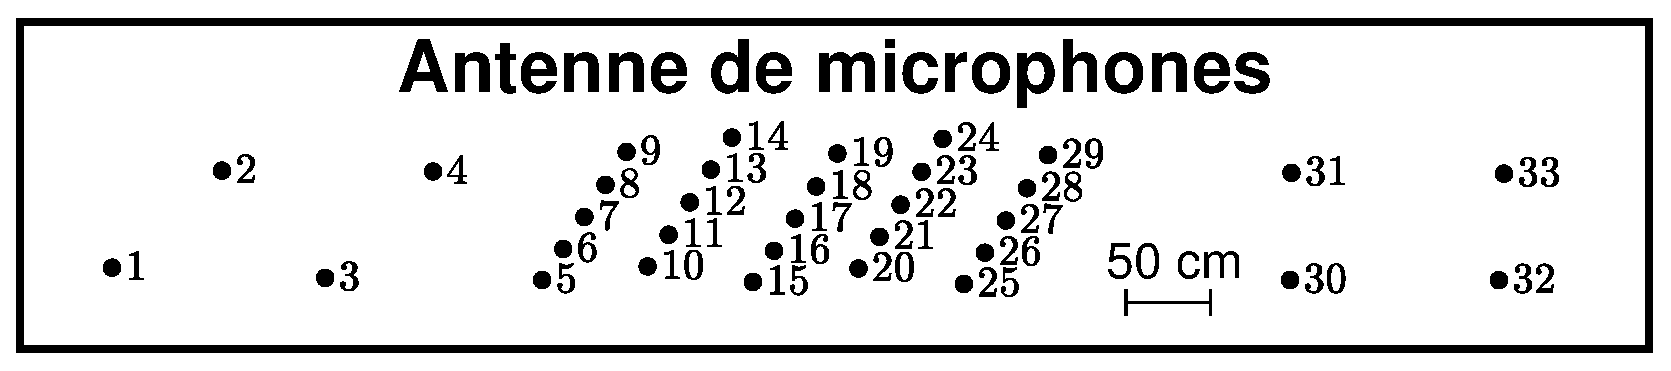
\includegraphics[width=4cm]{mic.eps}};
		\node[align=center,font=\scriptsize] (mic2) at ($(mic.east)+(2cm,0)$) { ${p}_1(f)$ \\$\dots$\\ ${p}_M(f)$};
		\draw[->,>=stealth] (mic.east) to ($(mic2.north west)-(0,1.8ex)$);
		\draw[->,>=stealth,dotted] (mic.east) to (mic2.west);
		\draw[->,>=stealth] (mic.east) to ($(mic2.south west)+(0,1.8ex)$);
	\end{tikzpicture}
	\vspace{1cm}
	\vfill
	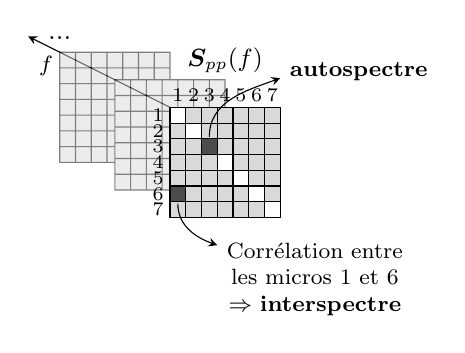
\begin{tikzpicture}		
		\uncover<5->{
		\draw[->,>=stealth] (0,\nbpas\pas) to ++($(-\nbpas\pas,\nbpas\pas/2)+(-2\pas,\pas)$) ;
		\node at ($(0,\nbpas\pas)+((-\nbpas\pas,\nbpas\pas/2)+(0,0.5em)$) {...};
		\node at ($(0,\nbpas\pas)+((-\nbpas\pas,\nbpas\pas/2)-(0.5em,0.5em)$) {\footnotesize $f$};
		\begin{scope}[transparency group,opacity=0.5]
			\draw[step=\pas,draw=black,fill=gray!30,thin,xshift=-\nbpas\pas,yshift=\nbpas\pas/2]  (0,0) grid (\nbpas\pas,\nbpas\pas) rectangle (0,0);
			\draw[step=\pas,draw=black,fill=gray!30,thin,xshift=-\nbpas\pas/2,yshift=\nbpas\pas/4]  (0,0) grid (\nbpas\pas,\nbpas\pas) rectangle (0,0);
		\end{scope}
		}
		\uncover<2->{
		\node at ($(0,\nbpas\pas)+(3.5\pas,3\pas)$) {\small $\bm{S}_{pp}(f)$};
		\draw [fill=gray!30] (0,0) rectangle ++(\nbpas\pas,\nbpas\pas) ;
		\draw[step=\pas,black,thin] (0,0) grid (\nbpas\pas,\nbpas\pas);
		\foreach \xtick in {1,...,\nbpas} { \node at (\xtick\pas-0.5\pas,\nbpas\pas+1ex) {\scriptsize\pgfmathprintnumber{\xtick}}; }
		\foreach \ytick [count=\ny from 1] in  {\nbpas,...,1} { \node at (-1ex,\ytick\pas-0.5\pas) {\scriptsize\pgfmathprintnumber{\ny}}; }
		\foreach \x in {1,...,\nbpas}{			
			\draw [fill=white] (\x\pas-\pas,\nbpas\pas-\x\pas) rectangle ++(\pas,\pas) ;			
		}
		}
		\uncover<3->{
			\draw [fill=black!70] (0\pas,1\pas) rectangle ++(\pas,\pas) ;
			\node (inter) at (0+0.5\pas, \pas+0.5\pas) {};
			\node[anchor=north west,align=center,font=\footnotesize] (inter2) at ($(inter)+(0.5cm,-0.5cm)$)  {   Corrélation entre \\  les micros 1 et 6\\ $\Rightarrow$  \bfseries interspectre};
			\draw[->,>=stealth] (inter) to [out=-90,in=160] ($(inter2.north west)-(0,1ex)$) ;
		}
		\uncover<4->{
			\draw [fill=black!70] (2\pas,4\pas) rectangle ++(\pas,\pas) ;
			\node (auto) at (2\pas+0.5\pas, 4\pas+0.5\pas) {};
			\node[anchor=north west,align=center,font=\footnotesize] (auto2) at (\nbpas\pas,\nbpas\pas+0.7cm)  {  \bfseries autospectre};
			\draw[->,>=stealth] (auto) to [out=90,in=200] ($(auto2.south west)+(0,1ex)$) ;
		}
			
	\end{tikzpicture}  
	\vfill 
\end{frame}

%%% CSM properties
%======================
%\section{CSM properties}
\begin{frame}[t]{Propriétés de la MI}
\centering
	
	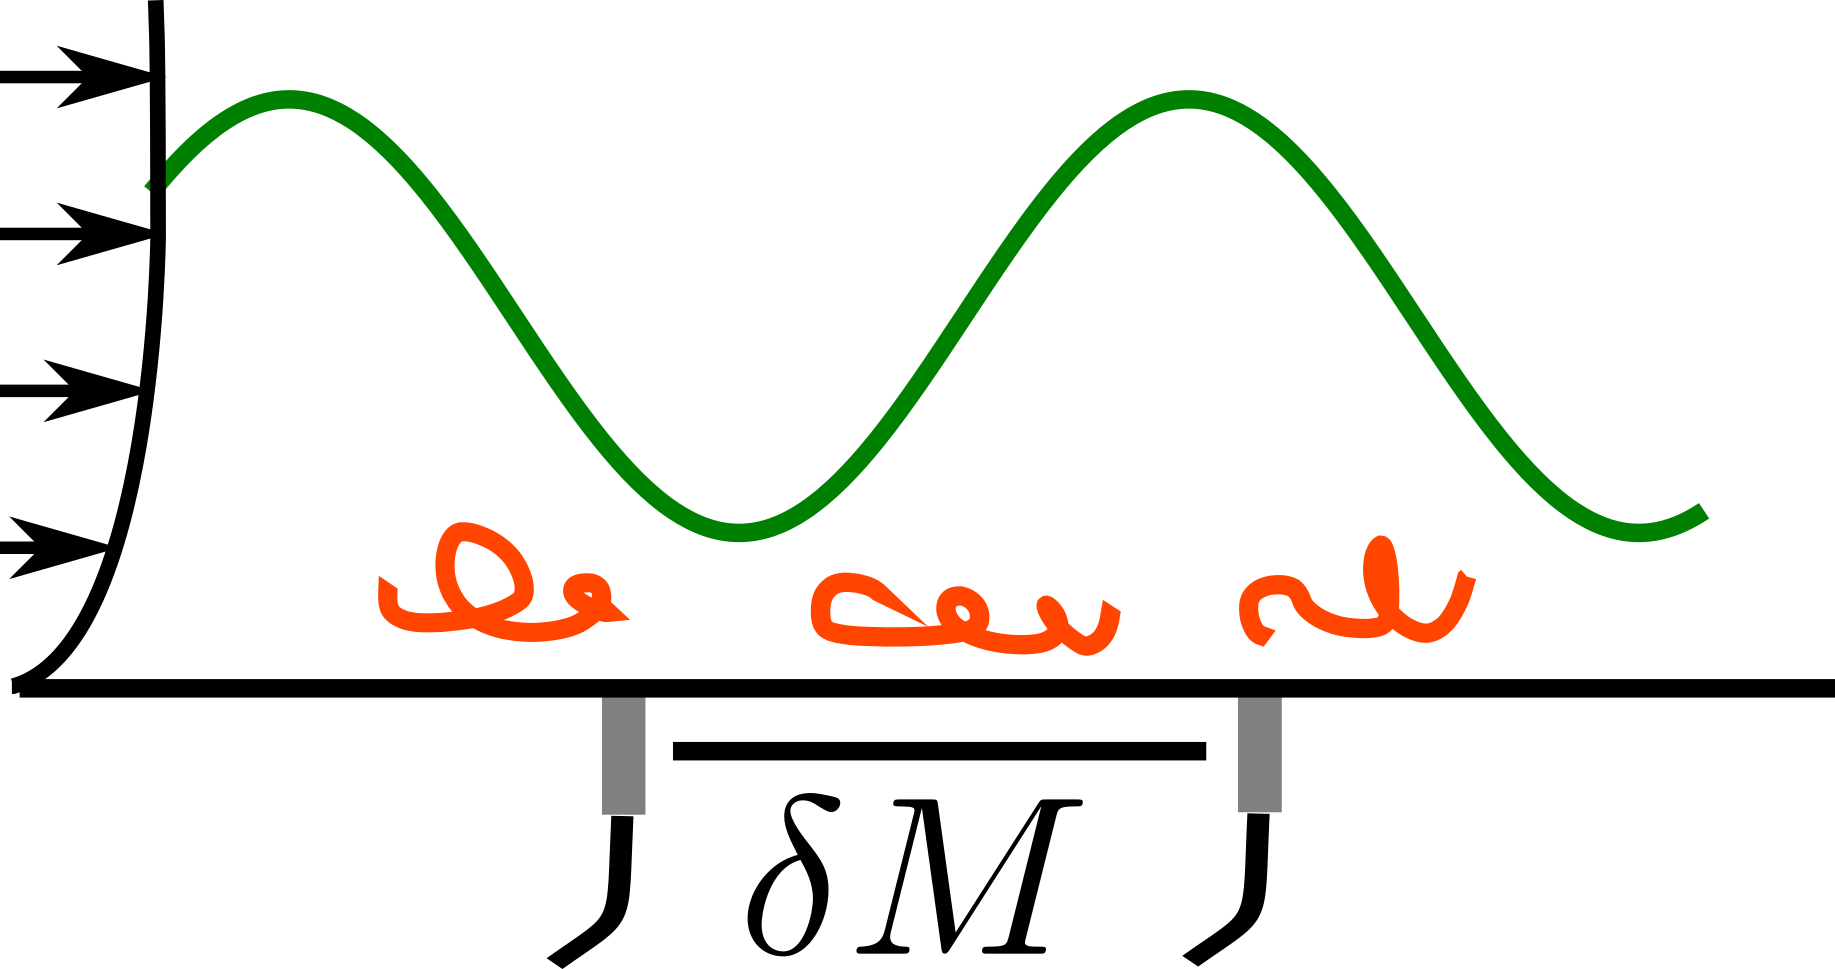
\includegraphics[width=3cm]{idee.png}

	\vfill

\begin{overlayarea}{\textwidth}{0.4\textheight}
	\alt<1-1>{\small Pour $i=1,\dots,I$ moyennes}{\small MI moyennées :}
	\only<1>{
	$$\underbracket[0.5pt]{~\bm{p}_i~}_{\text{spectres mesurés}} =\underbracket[0.5pt]{~\textcolor{source}{\bm{a}}_i~}_{\text{sources acoustiques}} + \underbracket[0.5pt]{~\textcolor{rouge}{\bm{n}}_i~}_{\text{bruit à retirer}} $$
	}
	\only<3->{$$\underbracket[0.5pt]{~\bm{S}_{pp}~}_{\text{MI mesurée}} =\underbracket[0.5pt]{ ~\textcolor{source}{\bm{S}_{aa}}~}_{\text{sources acoustiques}} +\underbracket[0.5pt]{\bcancel{~\textcolor{rouge}{\bm{S}_{nn}}~}}_{\parbox[t]{2cm}{\centering \text{\scriptsize bruit à retirer} \\ $\approx$ \scriptsize diagonale }} + \underbracket[0.5pt]{\bcancel{~\bm{S}_{an}+\bm{S}_{na}}}_{\parbox[t]{2cm}{\centering  \text{\scriptsize termes croisés}\\ $\rightarrow 0$ }}$$
	}	
	\only<2>{$$\underbracket[0.5pt]{~\bm{S}_{pp}~}_{\text{MI mesurée}} =\underbracket[0.5pt]{ ~\textcolor{source}{\bm{S}_{aa}}~}_{\text{sources acoustiques}} +\underbracket[0.5pt]{~\textcolor{rouge}{\bm{S}_{nn}}~}_{\parbox[t]{2cm}{\centering \text{\scriptsize bruit à retirer} \\ ~}}  + \underbracket[0.5pt]{~\bm{S}_{an}+\bm{S}_{na}}_{\parbox[t]{2cm}{\centering  \text{\scriptsize termes croisés}\\ ~ }}$$
	}
	
	
	
	\onslide<3->{
	\centering
	\setlength{\larg}{0.3cm}	
	 \setlength{\haut}{1.3cm}
	 \setlength{\tabcolsep}{0.7ex}
	 \hspace{-1.5cm}\tikz{
		 	\node at (0,0) (a) {};
		 	\draw [rectangle,main,line width=1pt,fill=main!10] (a)  rectangle  ++ (\larg,-\haut)  ; 	 
		 	%\draw[rectangle,main,line width=1pt,fill=main!10] (a)++(\larg+0.1cm,-0.5\haut+0.5\larg) rectangle ++(\larg,-\larg);
			\draw[main,rectangle,line width=1pt,fill=main!10] (a)++(1\larg+0.1cm,-0.5\haut+0.5\larg) rectangle ++(\haut,-\larg);
			\node at ($(a)+(2.5\larg+\haut,-0.5\haut)$) {$+$};
			\node at ($(a)+(-\larg,-0.5\haut)$) {$=$};
		} 
		\tikz{
			\draw[main,line width=1pt]  (-0.9cm,0) rectangle ++(\haut,-\haut); 
			\draw[line width=1pt,main] (-0.9cm,0) to ++(\haut,-\haut);
		}	
		}
\end{overlayarea}	

	\begin{itemize}
		\setlength{\itemindent}{1cm}
		\item<3-> Signal \textcolor{source}{acoustique} corrélé : {\bfseries MI à rang réduit}\\ \centering peu des monopoles équivalents
		\item<3-> \textcolor{rouge}{Bruit} faiblement corrélé : {\bfseries MI diagonale}\\		
	\end{itemize}
\end{frame}


\section{Analyse Factorielle Probabiliste}
\subsection*{Modèle statistique}
\begin{frame}{\insertsectionhead}
	\vfill
	\begin{itemize}
        		\item<1-> \textbf{Modèle statistique}\\    ~\\    		
        		\hspace{-2em}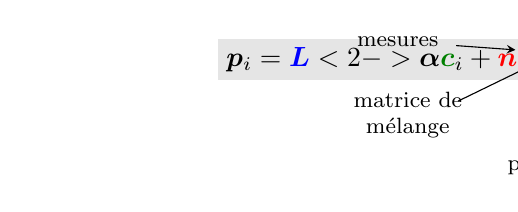
\begin{tikzpicture}[remember picture]
			\colorbox{gray!20}{$\tikzmark{p}\bm{p}_i = \tikzmark{L}\textcolor{blue}{\bm{L}}
			\uncover<2->{\tikzmark{alpha}\bm{\alpha}}
			 \tikzmark{c}\textcolor{green}{\bm{c}}_i + \tikzmark{n}\textcolor{red}{\bm{n}}_i$}
			
			%p
			\node (pdescr) [below left=-0.5cm and 1cm of p, align=center,font=\footnotesize]{
				mesures
			};
			\draw[->,>=stealth] (pdescr) -- ($(p.east)+(-7pt,6pt)$);
			
			% L
			\node(Ldescr) [below left=0.2cm and 0.8cm of L,align=center,font=\footnotesize] {
				 matrice de\\ mélange
			};
	    		%\draw[] (Ldescr.east) to [in=-90,out=45]  (L.south) ;
	    		\draw[->,>=stealth] ($(Ldescr.east)+(-5pt,5pt)$) to ($(L)+(-2pt,0)$);
	    		
	    		%alpha
	    		\uncover<2->{
	    		\node (adescr) [below=of alpha,font=\footnotesize,align=center]{poids};
	    		\draw[->,>=stealth] (adescr) to ($(alpha.south)$);
	    		}
	    		
	    		% c
	    		\node(cdescr) [below right  =0.3cm  and 0.8cm of c , align=center,font=\footnotesize]{
	    			facteurs\\latents
	    		};
	    		\draw[->,>=stealth] (cdescr) to ($(c.south)+(2pt,0)$);
	    		
	    		% n
	    		\node(ndescr) [below right=-0.5cm and 1cm of n,align=left,font=\footnotesize]{
	    			bruit (+erreurs)
	    		};
	    		\draw[->,>=stealth] (ndescr.west) to ($(n.east)+(11pt,6pt)$);
		\end{tikzpicture}
		
		\begin{itemize}
		        \item Représente les principales corrélations avec quelques paramètres (proche de l'ACP) \\
		        $\hookrightarrow$ MI à rang réduit
		        \item Modèle de bruit anisotrope\pause
		        \item Renforce la parcimonie pour réduire le nombre de facteurs\\
		        $\hookrightarrow$  Compression de donnée
		\end{itemize}
	\end{itemize}
	\vfill
        	\begin{overlayarea}{\textwidth}{0.5\textheight}
        	\onslide<3->{
	\begin{itemize}        		
        		\item \textbf{Approche bayésienne : } une densité de probabilité par paramètre\\[1ex]
        		\renewcommand{\arraystretch}{1.5}    		
        		\hspace{-1cm}\begin{tabular}{|c|c|c|c|}
        		\hline
        		$\textcolor{blue}{\bm{L}}\sim\mathcal{N}_{\mathbb{C}}(0,\diag{\frac{1}{K}})$& 
		$\textcolor{green}{\bm{c}}_i\sim\mathcal{N}_{\mathbb{C}}(0,\diag{\bm{\gamma}^2})$&
		$\textcolor{rouge}{\bm{n}}_i\sim\mathcal{N}_{\mathbb{C}}(0,\diag{\bm{\sigma}_n^2})$&
		$\bm{\alpha}\sim\mathcal{E}(a_\alpha)$\\\hline
		\end{tabular}       \\[0.5ex]
		+ hyper-paramètres : $\bm{\gamma}^2, \bm{\sigma}^2\sim\mathcal{IG}(\bm{a}_{\gamma,\sigma},\bm{b}_{\gamma,\sigma})$\\[1ex]      	
%		\pause			 
%        		   \vfill     		
%        		\item \textbf{Solved using MCMC algorithm} (Gibbs sampling)\\
%		\small Iterative draws in the marginal conditional distributions of each parameter\normalsize
%		\pause		
%        		 \vfill 
%        		 \vspace{-0.5em}
%        		 \item \textbf{Finally}, signal CSM: 
%        		 \hspace{4ex}\parbox{0.3\textwidth}{
%        		 $$\bm{\hat{S}}_{aa}=\frac{1}{N_s}\sum_{i=1}^{N_s}\textcolor{blue}{\bm{L}}\textcolor{green}{\bm{c}}_i\textcolor{green}{\bm{c}}^H_i\textcolor{blue}{\bm{L}}^H$$        
 %       		}
		 
	\end{itemize}
	}		
	\end{overlayarea}	
\end{frame}

\begin{frame}{\insertsectionhead ~--~ Optimisation}
	\centering
	\begin{tikzpicture}
		\node (pic) {\fbox{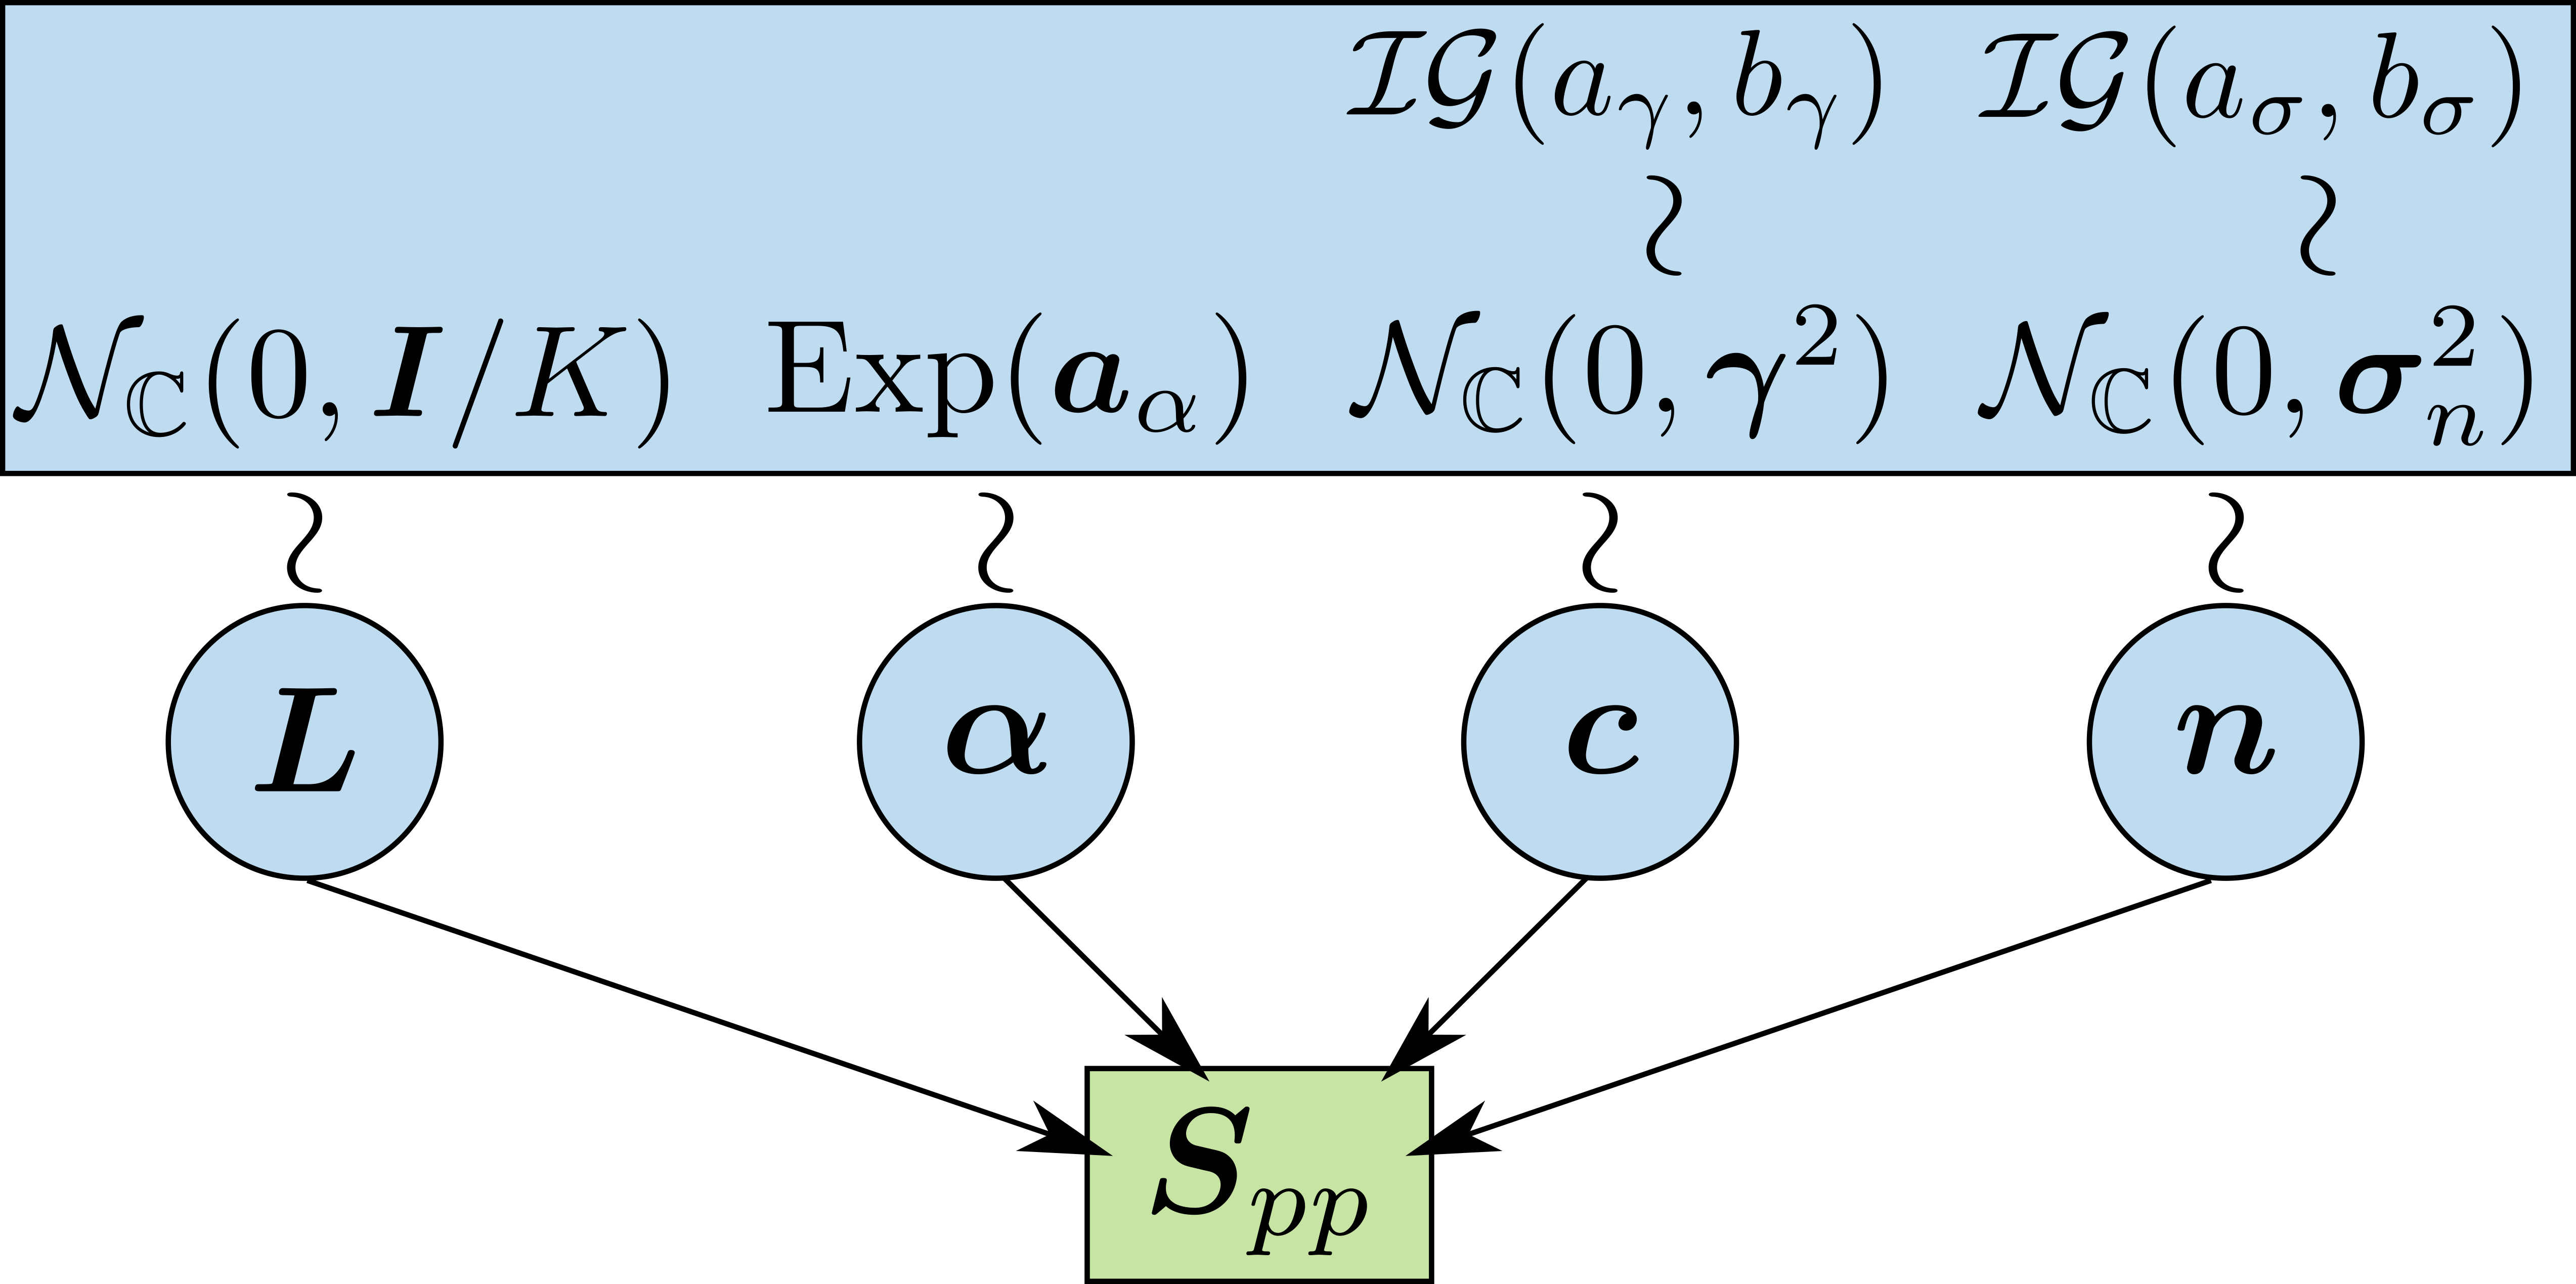
\includegraphics[width=0.44\textwidth]{modele.png}}};
		\node (mod) [right=0.7 of pic,align=center] {
			\textbf{Modèle paramétrique}: $\mathcal{M}(\bm{\theta})$\\
			\small avec $\bm{\theta} = \left\{\bm{L},~\bm{\alpha},~\bm{c},~\bm{n},~\bm{a}_{\gamma,\alpha,\sigma},~\bm{b}_{\gamma,\alpha,\sigma}\right\}$
		};
		\draw[->,>=stealth,line width=1pt] (pic) to (mod);
	\end{tikzpicture}
	\vfill	
	\begin{tabular}{c c}
		\textbf{Étape d'optimisation }:&
		$\boxed{ \displaystyle  \bm{\theta} =\underset{\bm{\theta}}{\arg\!\max} \underbrace{p\left( \bm{\theta} \mid \bm{S}_{yy}\right)}_{ \text{\pbox{7cm}{\centering \normalsize fonction objectif}}}}$ %fr :  fonction obectif	
	\end{tabular}
	\vfill
	La fonction objectif est la probabilité postérieure $\rightarrow$ pas de forme explicite\\
	$\hookrightarrow$ approximation avec des méthodes numériques
	%The fitness function is the posterior probability $\rightarrow$ has no close form\\
	%$\hookrightarrow$ approximation with numerical methods
	


\end{frame}





\newlength{\wg} \setlength{\wg}{0.4\textwidth}
\begin{frame}{\insertsectionhead~-- Optimisation}
\textbf{Maximisation de la distribution a posteriori}\\
{\itshape $\hookrightarrow$Trouver les paramètres optimaux  qui expliquent au mieux les données\\
$\hookrightarrow$ Méthode : l'échantillonneur de Gibbs}
\vfill
\begin{overlayarea}{\textwidth}{0.5\textheight}
\centering
\includegraphics<1>[trim=-1.66cm 0 0 0, clip,height=\wg,angle=-90]{model2.pdf}
\includegraphics<2>[trim=-1.66cm 0 0 0, clip,height=\wg,angle=-90]{model0.pdf}
\includegraphics<3>[trim=-1.66cm 0 0 0, clip,height=\wg,angle=-90]{model3.pdf}
\includegraphics<4>[trim=-1.66cm 0 0 0, clip,height=\wg,angle=-90]{model4.pdf}
\includegraphics<5>[trim=-1.66cm 0 0 0, clip,height=\wg,angle=-90]{model5.pdf}
\includegraphics<6>[trim=-1.66cm 0 0 0, clip,height=\wg,angle=-90]{model6.pdf}
\includegraphics<7>[trim=-1.66cm 0 0 0, clip,height=\wg,angle=-90]{model7.pdf}
\includegraphics<8->[height=\wg+0.002\textwidth,angle=-90]{model8.pdf}
\end{overlayarea}
\vfill
\onslide<9->{
	\centering
	\begin{tabular}{c c c c c c}
	MI mesurée && MI signal && MI bruit\\
	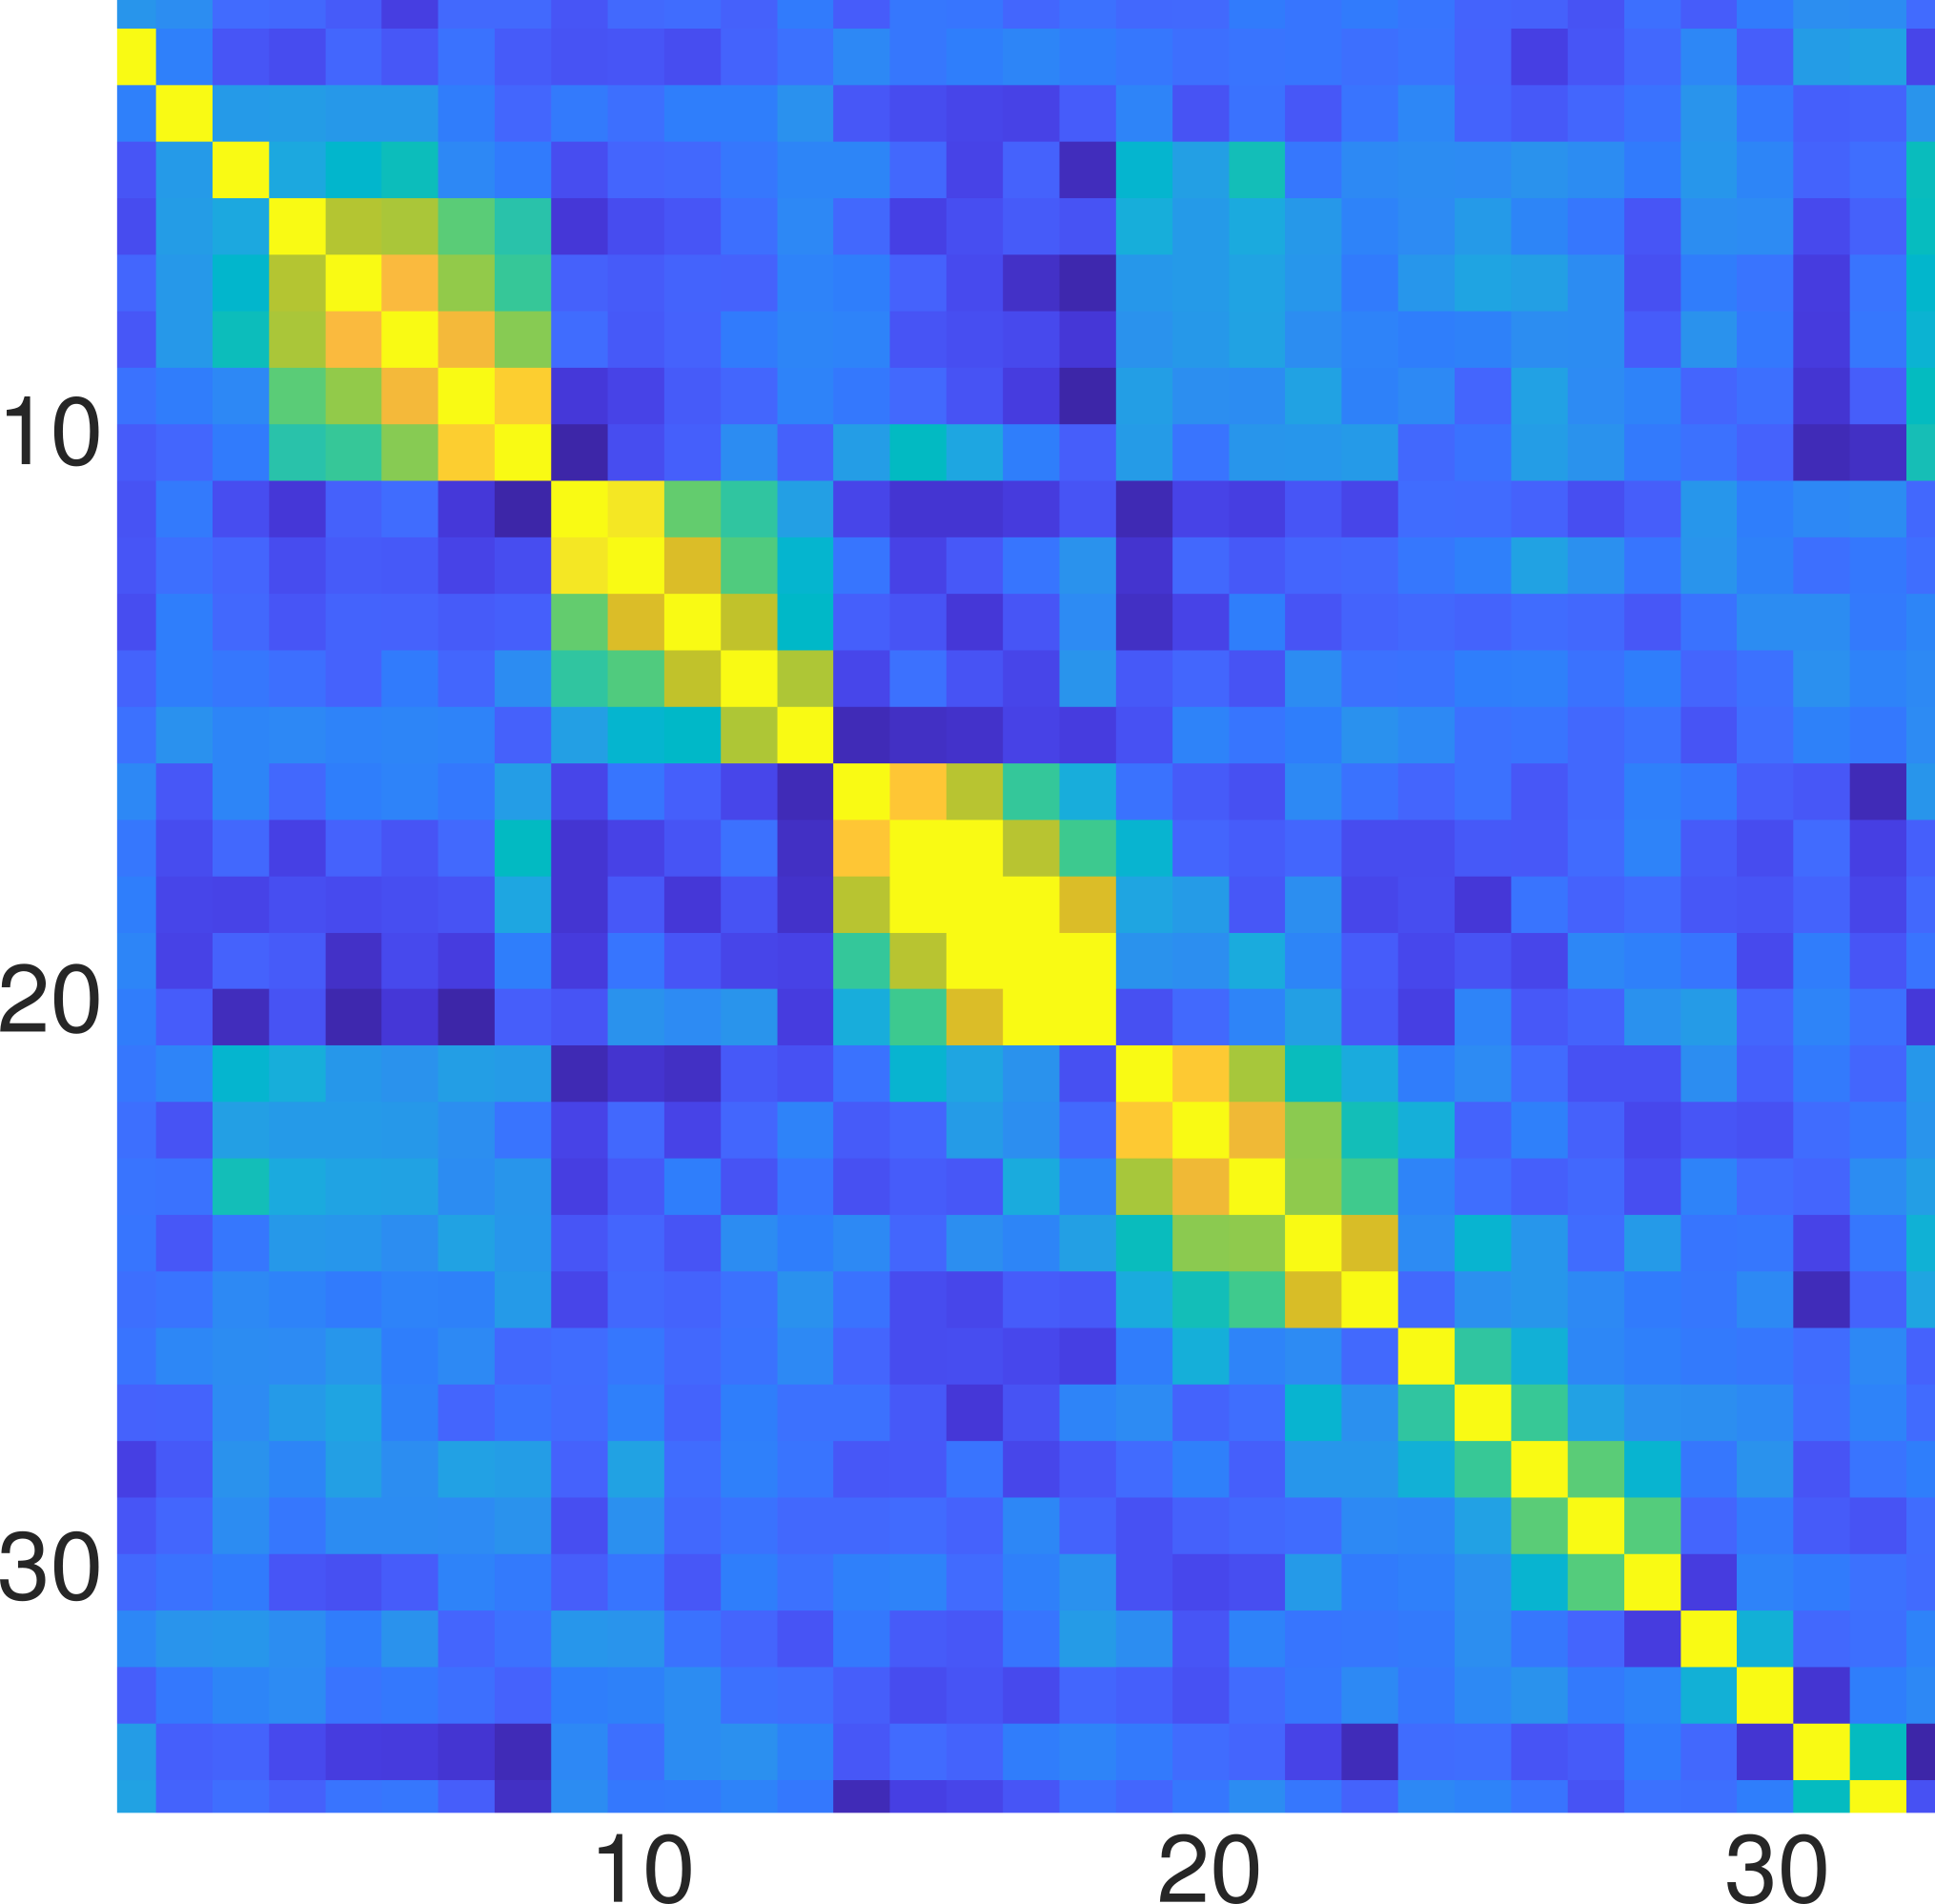
\includegraphics[valign=m,width=0.18\textwidth]{csm.png} &= & 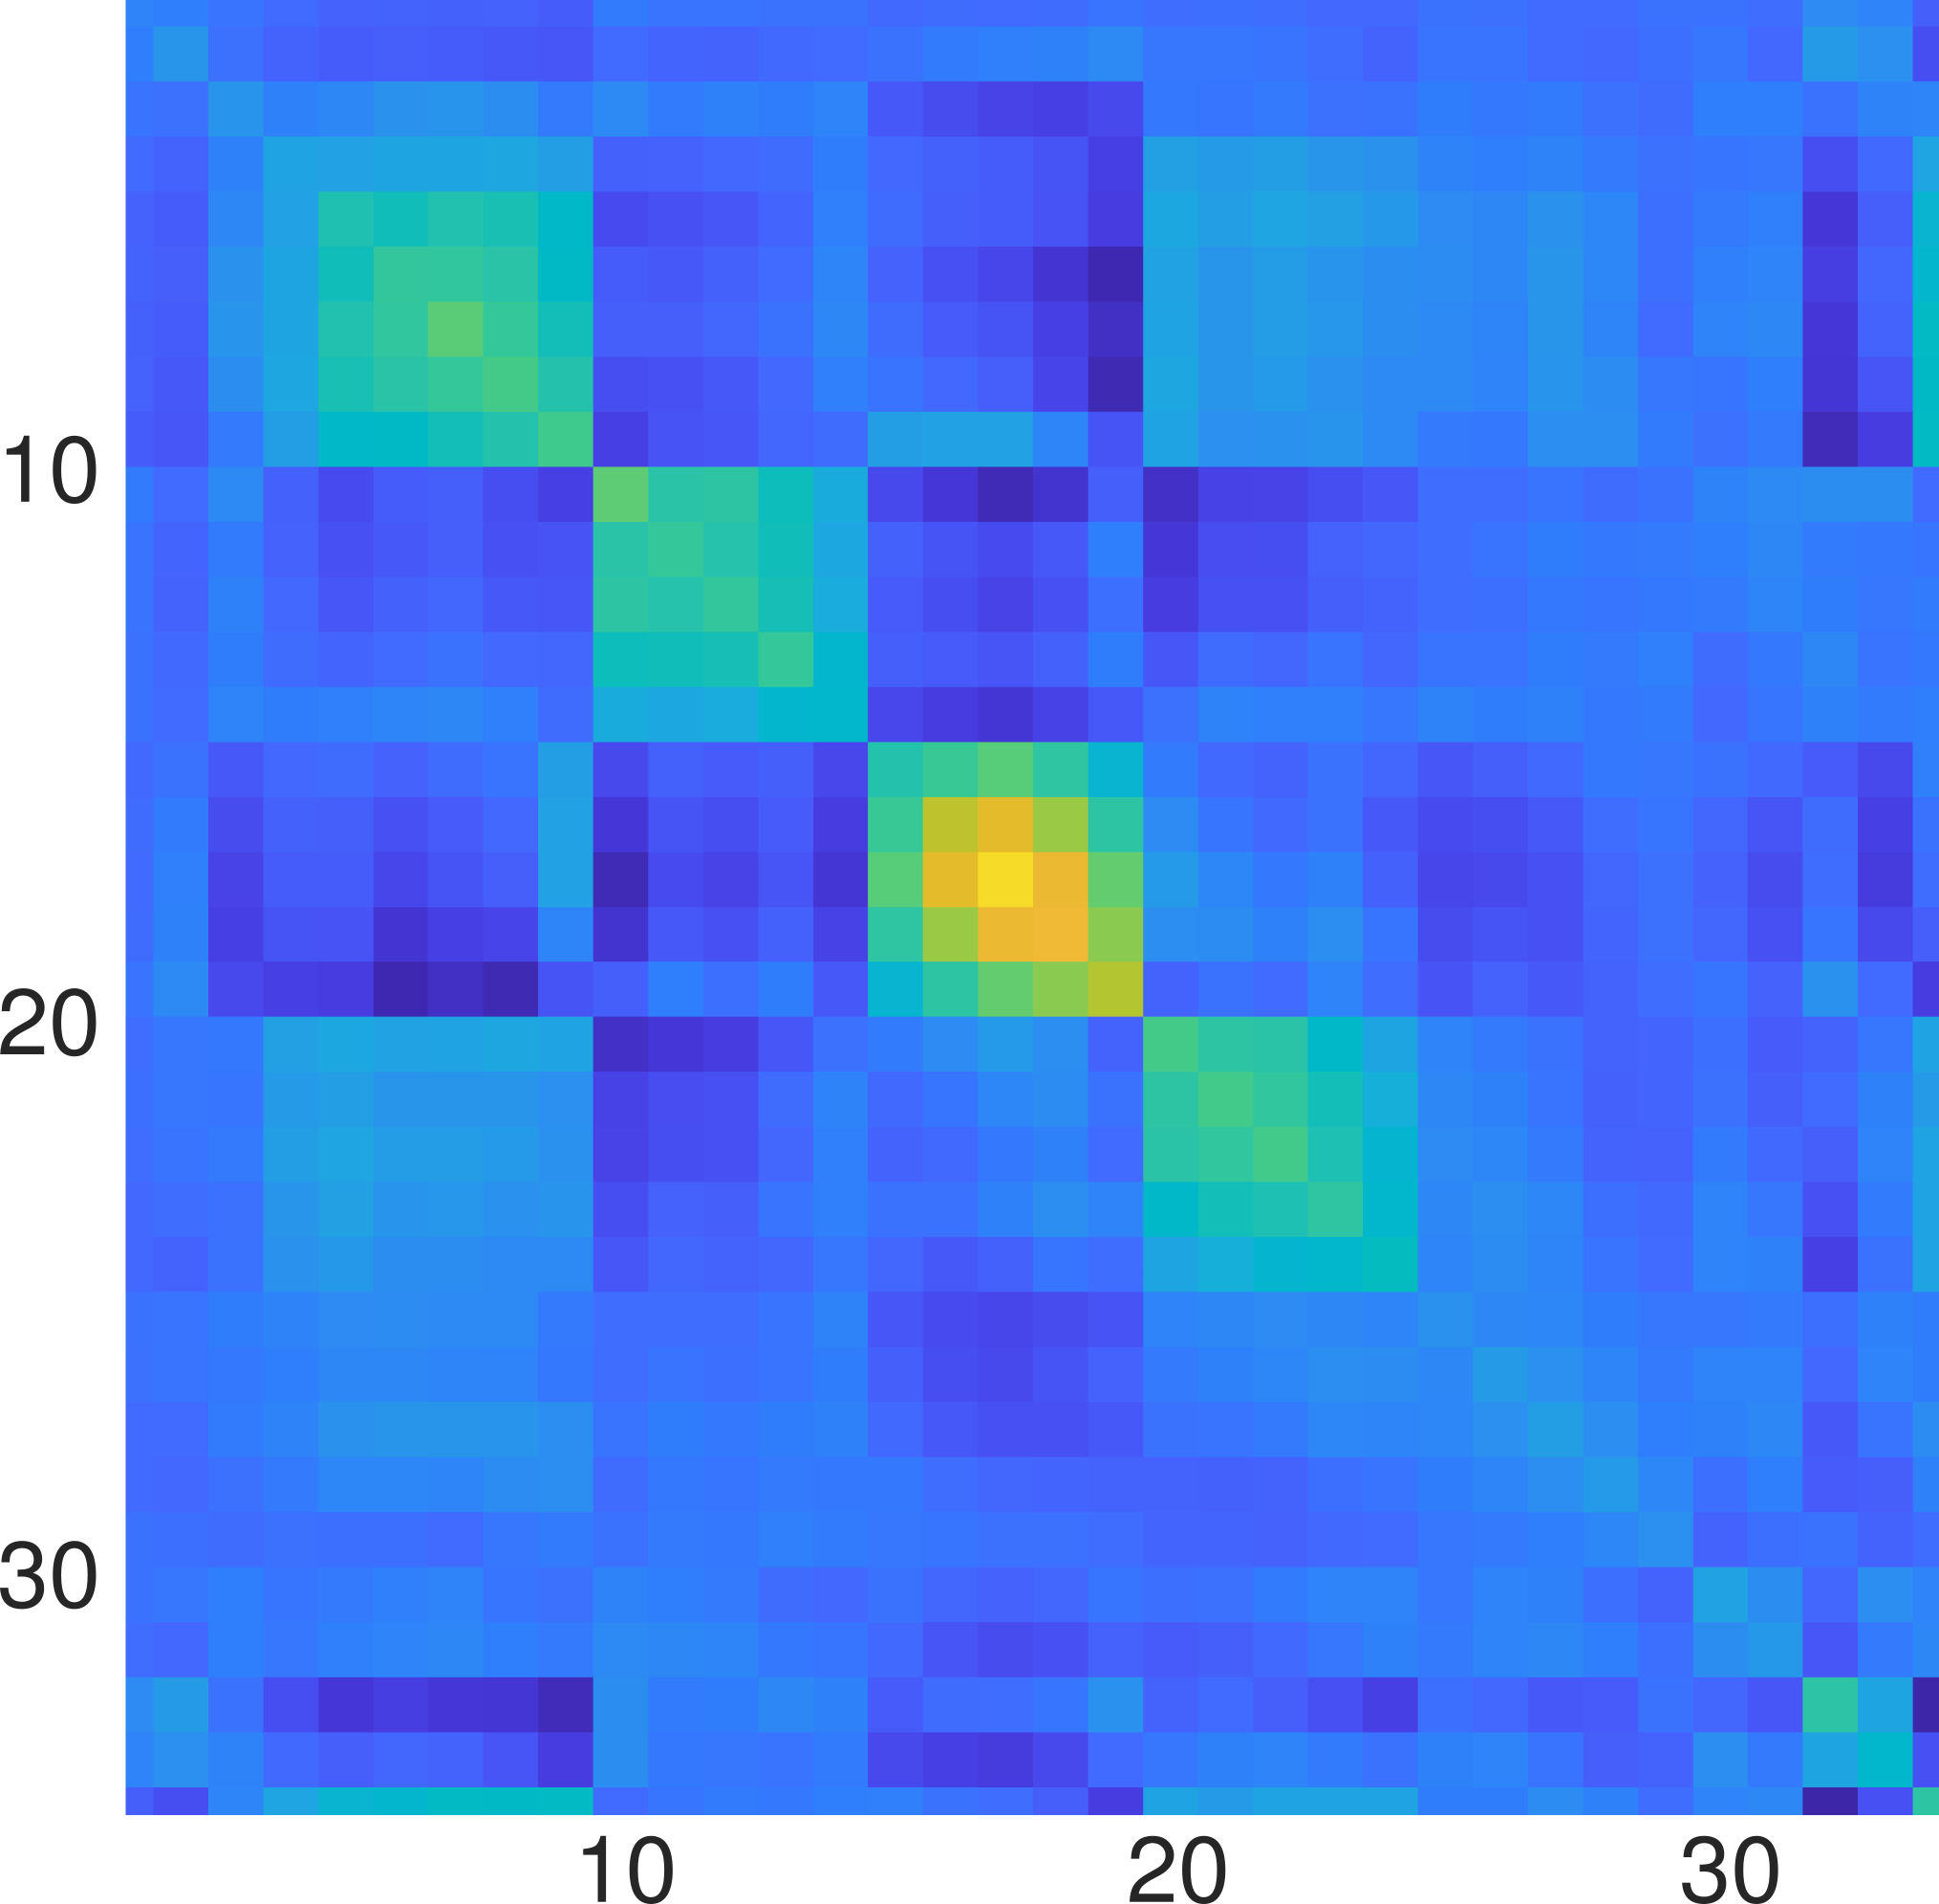
\includegraphics[valign=m,width=0.18\textwidth]{signal.png} & +&  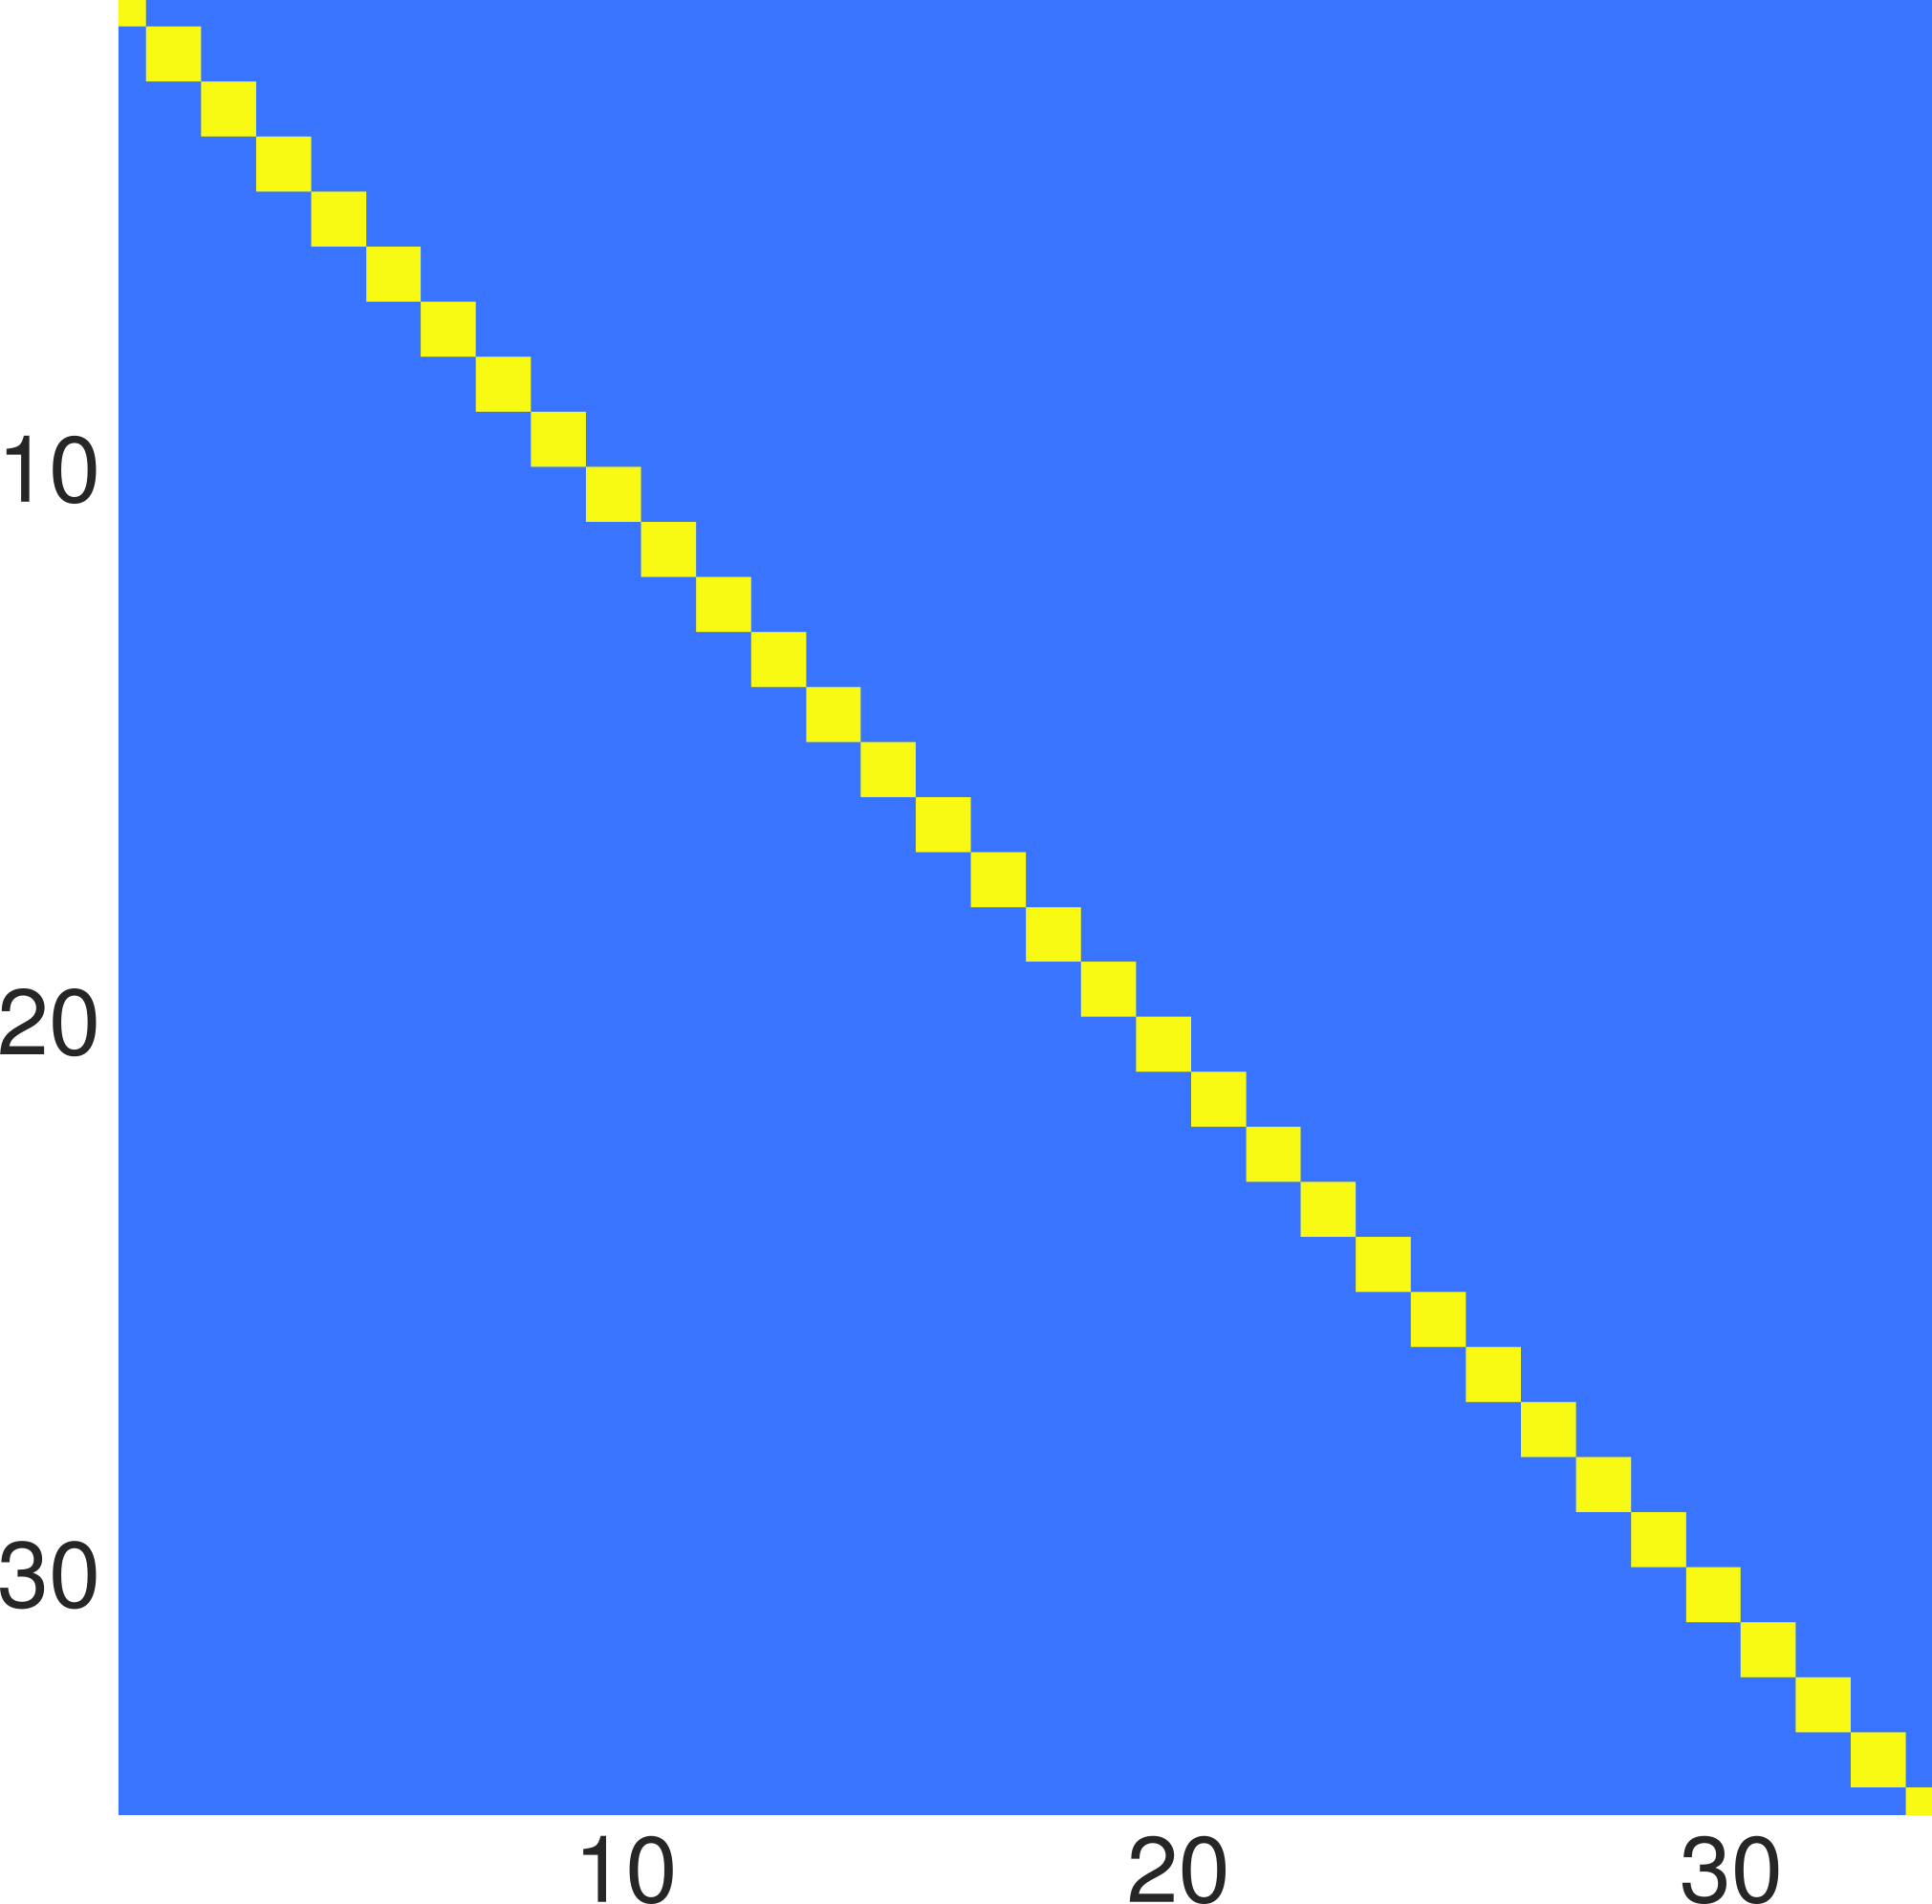
\includegraphics[valign=m,width=0.18\textwidth]{bruit.png} & \pbox{0.2\textwidth}{\centering \footnotesize Exemple de mesures en vol}\\
	\end{tabular}
}
\end{frame}

\begin{frame}{\insertsectionhead}
\vfill
\onslide<1->{
\hspace{-0.5cm}\begin{minipage}[t]{0.55\textwidth}
~\centerline{\resizebox{0.5cm}{!}{\circled{\textbf{+}}}} \\
\begin{itemize}
        \item[$\bullet$] Échantillonneur de Gibbs :
        \begin{itemize}
   	     \item intègre les connaissances a priori
   	     \item fournit un intervalle de crédibilité
   	     \item optimisation globale
	\end{itemize}
	\item[$\bullet$] AFP :
	\begin{itemize}
   	     \item la MI conserve un sens physique
   	     \item compresse les données
   	     \item  aucun paramètre à régler
   	     \item  modèle flexible
   	     \item possibilité de prendre en compte plusieurs configurations
	\end{itemize}
\end{itemize}
\vfill
\end{minipage}
}
\hfill
\pause
\begin{minipage}[t]{0.45\textwidth}
~\centerline{\resizebox{0.5cm}{!}{\circled{\raisebox{-1ex}{\textbf{$\:$-$\:$}}}}}\\[1ex]
\begin{itemize}
        \item[-] \small Sensibilité au choix des a priori \\ not. quand le problème est mal conditionné
        \item[-]  \small Coûts de calcul élevés
\end{itemize}
\vfill
\end{minipage}\\
\vfill
\end{frame}


\section{Débruitage référencé}
\begin{frame}{\insertsectionhead}

\textit{\small Hypothèse : pas de bruit extérieur (couche limite) sur les micros de référence}\\[1.5ex]

{\footnotesize
$\left.
\begin{tabular}{l l}
	$\bm{y}$ &: signaux à débruiter\\
	$\bm{r}$ &: signaux de référence non-bruités \\ &(ex : intérieur de cabine)
\end{tabular}
\right\} \text{acquis simultanément} $\\
\begin{tabular}{l l}
	 $\bm{a}$ & : signaux débruités
\end{tabular}
}
\vfill
\parbox{0.45 \textwidth}{
\hfill $\displaystyle \boxed{    \bm{S}_{aa} = \bm{S}_{yr}\bm{S}_{rr}^{-1}\bm{S}_{ry}}$
}
$\rightarrow$\parbox{0.4\textwidth}{\centering  Généralisation des\\ spectres cohérents}
\vfill
\pause

\rule{\textwidth}{0.4pt}
\begin{minipage}[t]{0.4\textwidth}
\small
~\\~\centerline{\resizebox{0.5cm}{!}{\circled{\textbf{+}}}} \\[-1ex]
\begin{itemize}
	\item Simple à implémenter
	\item Faible coût de calcul
\end{itemize}
\end{minipage}
\hfill
\begin{minipage}[t]{0.55\textwidth}
\small
~\centerline{\resizebox{0.5cm}{!}{\circled{\raisebox{-1ex}{\textbf{$\:$-$\:$}}}}}\\[-1ex]
\begin{itemize}
	\item signaux de référence : non bruités \\ (ou bruit décorrélé)
	\item nécessite des mesures simultanées supplémentaires
	\item les seuils de cohérence dépendent
	\begin{itemize}
        		\item de la longeur des signaux
       		 \item du nombre de références
	\end{itemize}
\end{itemize}
\end{minipage}
\vfill
\end{frame}



\section{Application en cas réel}
\begin{frame}{\insertsectionhead}
	\begin{tikzpicture}[remember picture, overlay]
		\node[yshift=-2cm,xshift=-4.5cm,right] (a) at (current page) {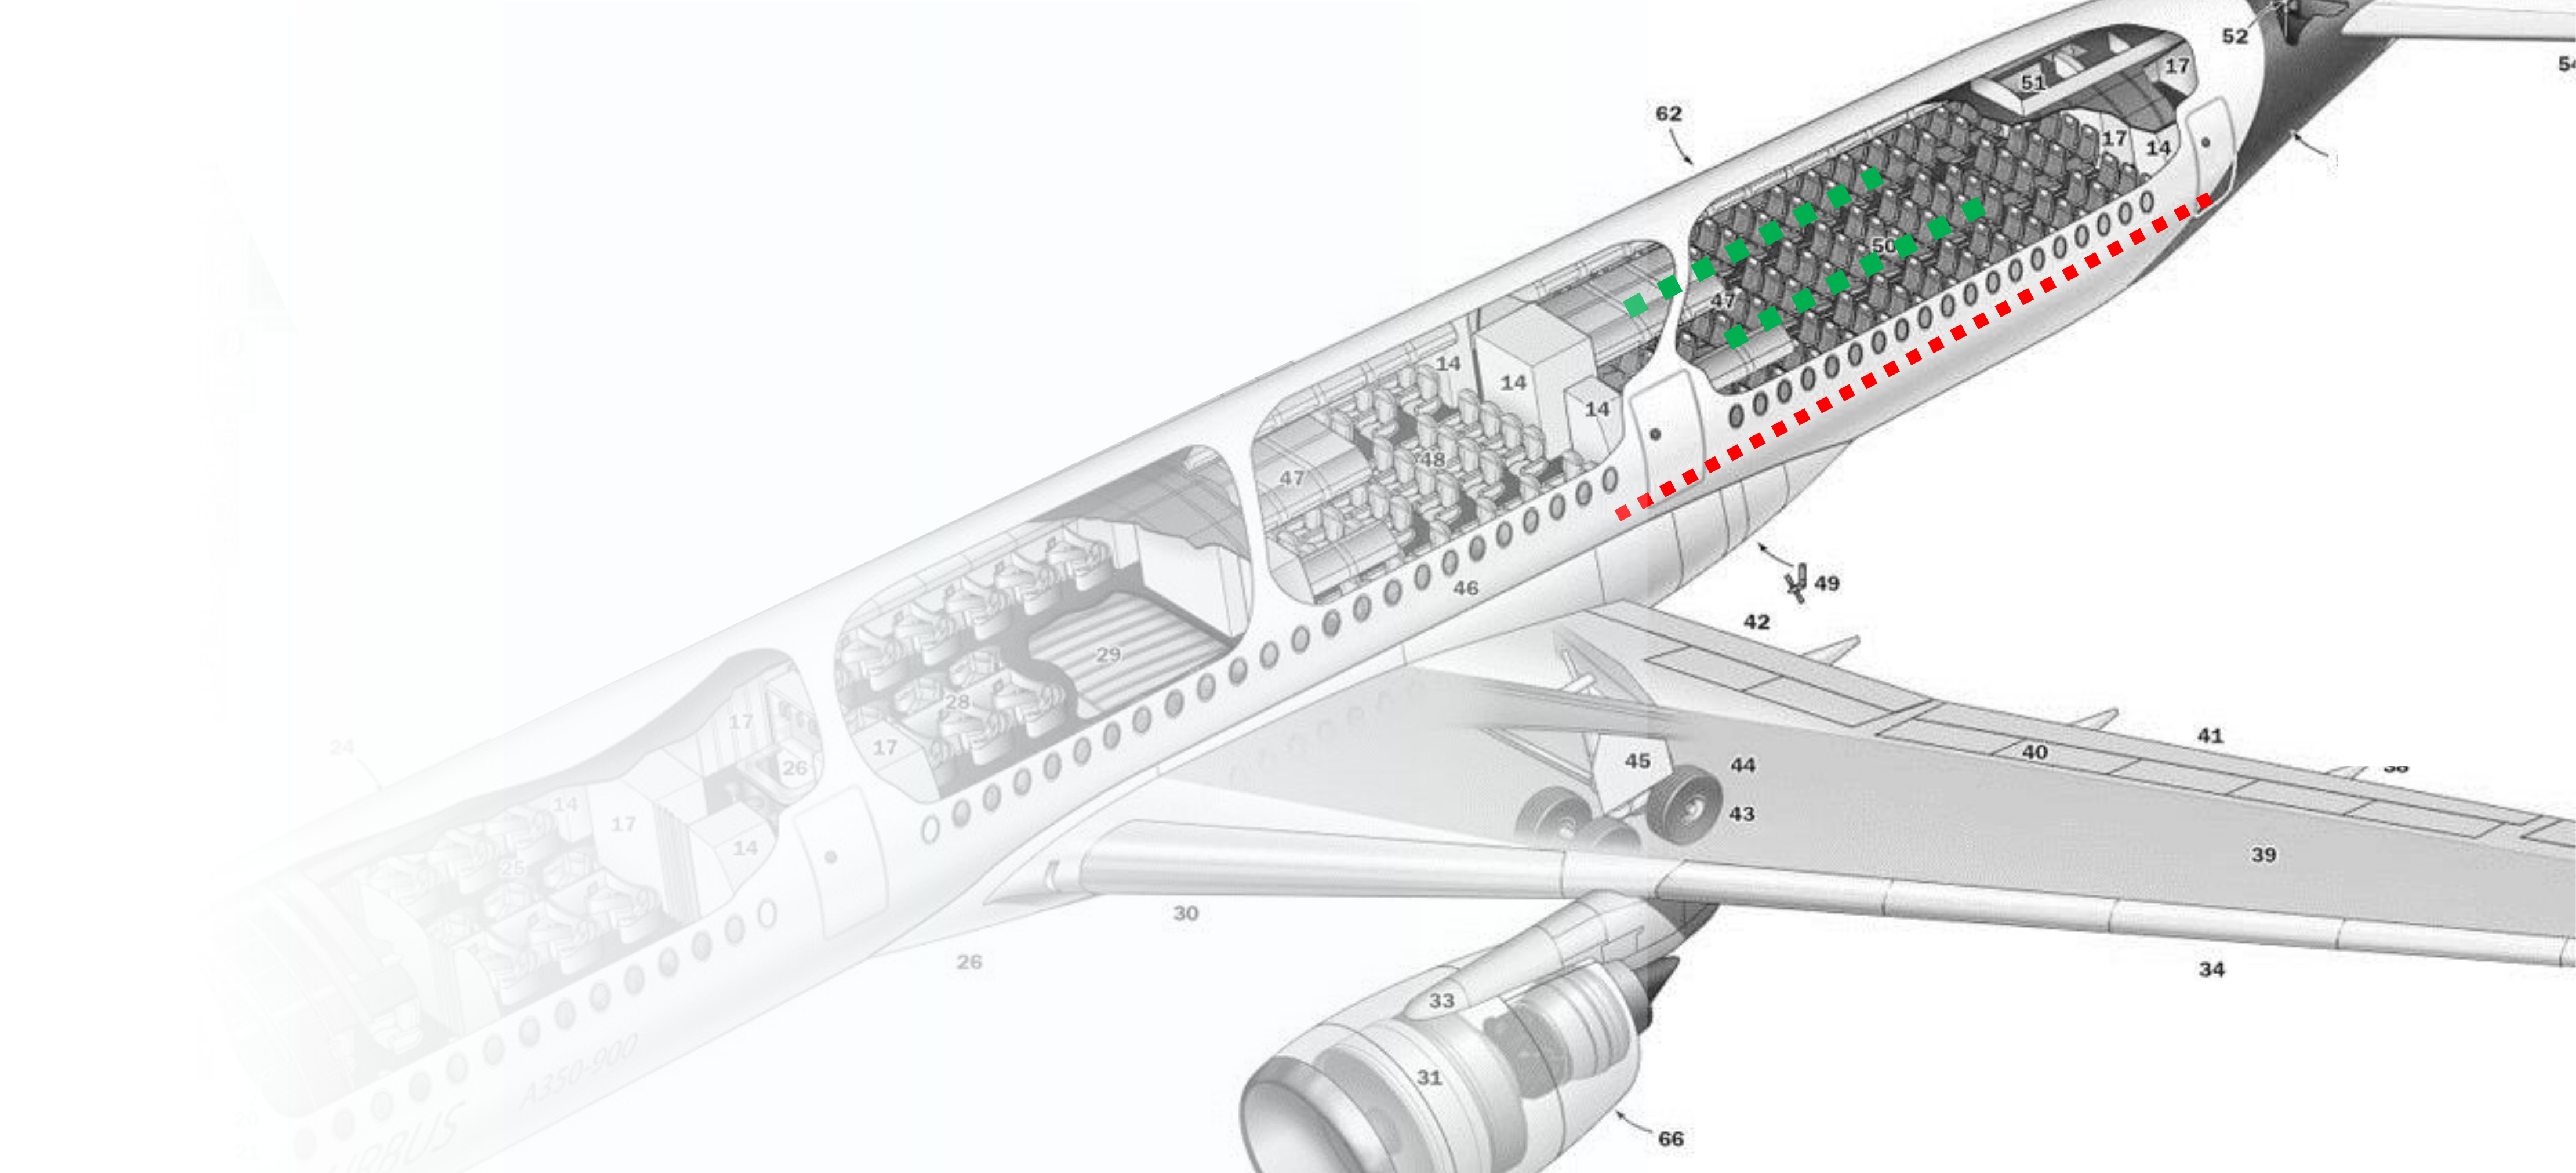
\includegraphics[width=\textwidth]{airbus/setup.png}};
		\node at ($(current page)-(0.5cm,0.2)$) {\parbox{10cm}{
		\begin{itemize}
	        		\item  Essais en vol
	        		\item Conditions réalistes de vol : Mach 0.85
	        		\item 6 régimes moteur dont 1 bruit de fond
	        		\item 35 microphones externes, sur le fuselage \tikzmark{ext}
	        		\item 14 microphones dans la cabine \tikzmark{int}
	        		\item MI :
	        		\begin{itemize}
	       		 	\item résolution : 4 Hz
	       		 	\item durée d'acquisition : 60 sec
	       		 	\item fenêtre de Hanning
	       		 	\item overlap : 70\%, éq. à 500 segments
			\end{itemize}		
			\item Bruits :
			\begin{itemize}
        				\item couche limite à l'extrérieur
        				\item ventilation à l'intérieur
			\end{itemize}
		\end{itemize}
		\vspace{1.5cm}
		}};
		\draw[->,>=stealth,rouge,line width=1pt] ($(ext)+(0,1.5ex)$) [out=0,in=110] to ($(a)+(3.2cm,1.5cm)$);
		\draw[->,>=stealth,source,line width=1pt] ($(int)+(0,1.5ex)$)  to ($(a)+(1.2cm,1.4cm)$);% [out=-45,in=135]
	\end{tikzpicture}
\end{frame}

\captionsetup[subfigure]{labelformat=empty}
\begin{frame}{\insertsectionhead}
Autospectres zoomés basses-moyennes fréquences\\[-2em]

\parbox{\textwidth}{
	\begin{figure}
		{\centering
		\subfloat[\scriptsize \itshape Mesure brute]{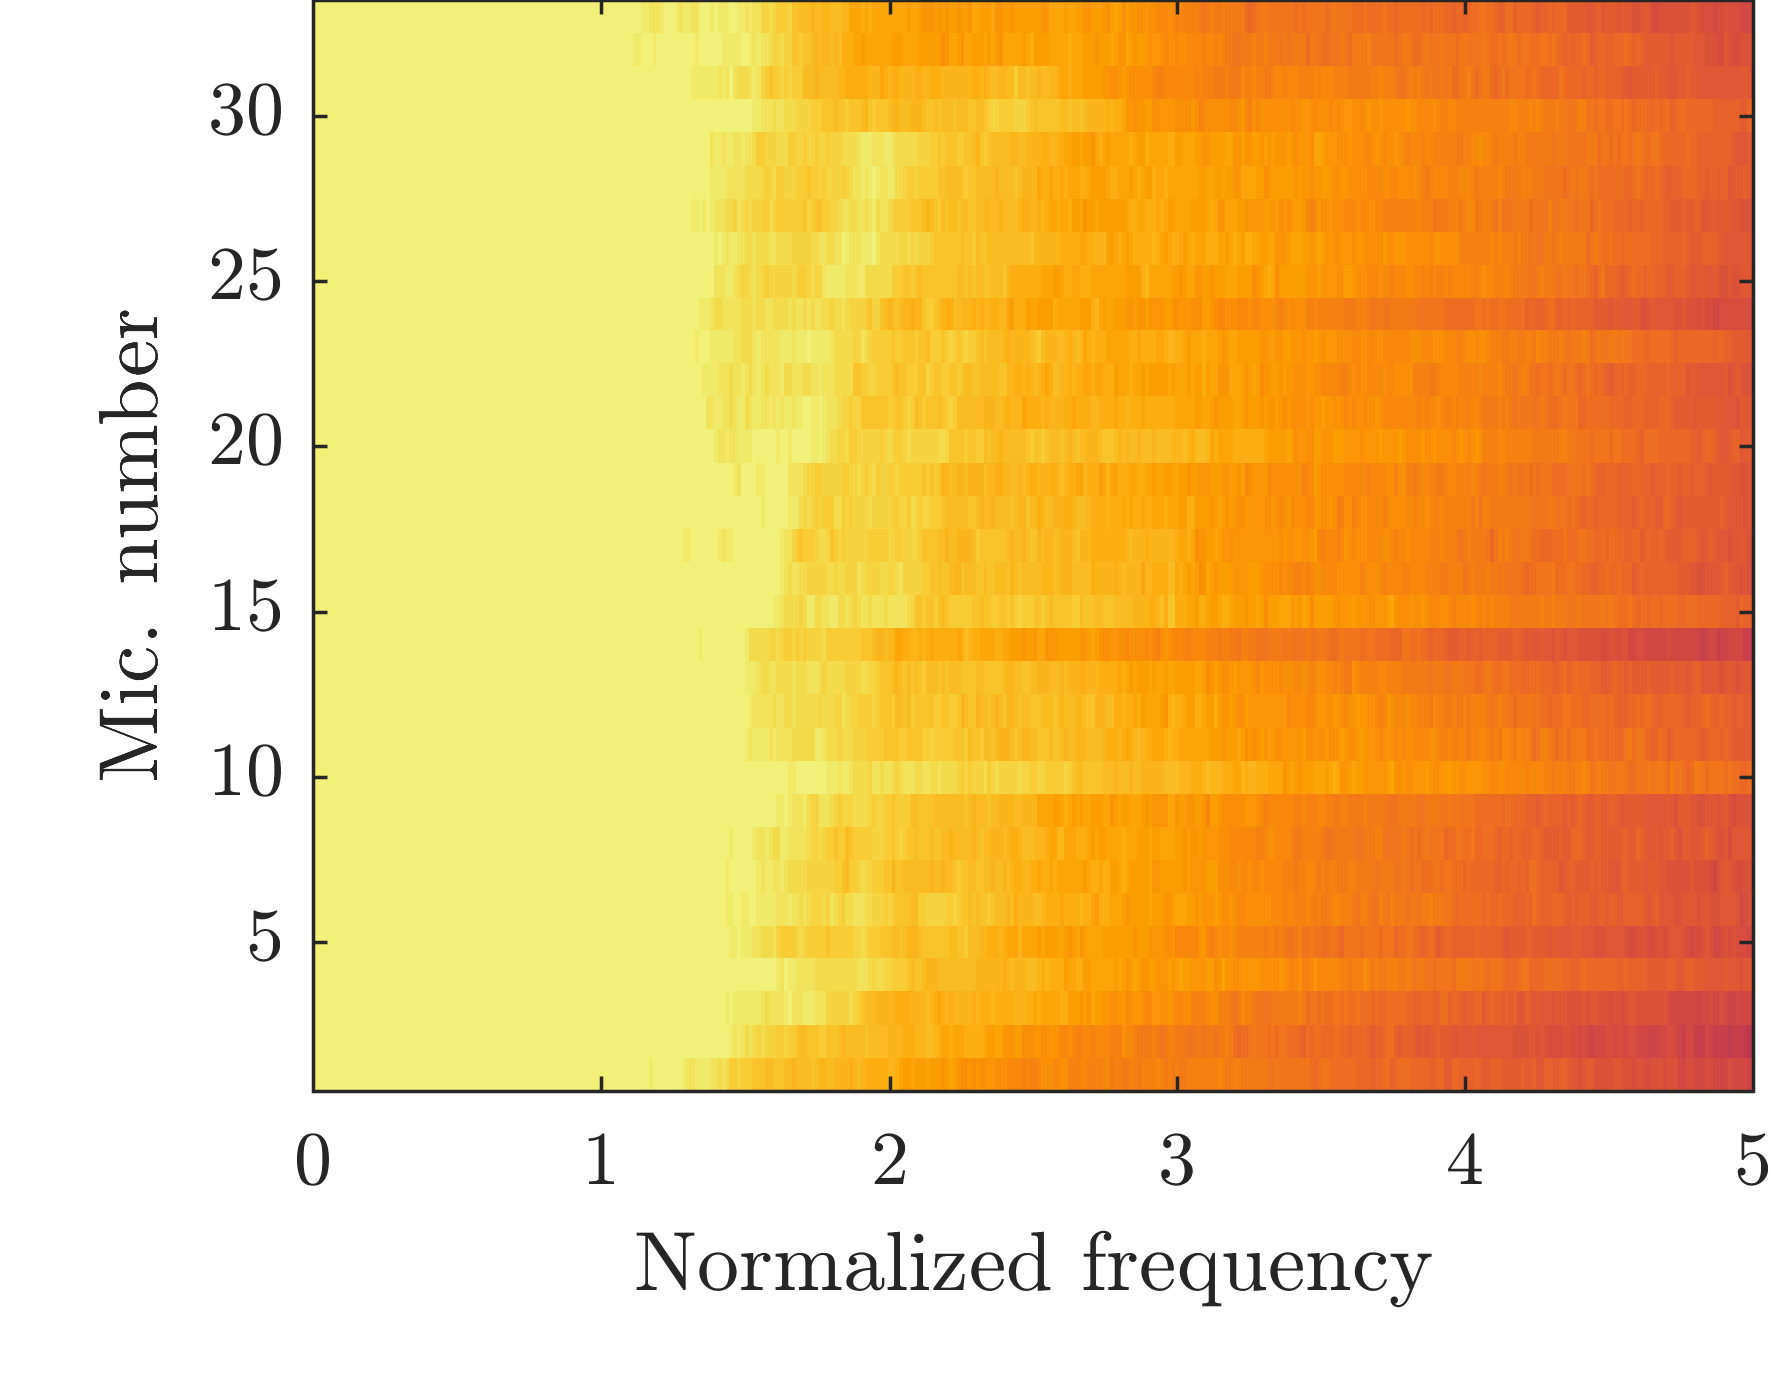
\includegraphics[trim = 2ex 1ex 0 0,clip, width=0.32\textwidth]{./airbus/as_raw.png}}%Raw (high engine speed)
		\subfloat[\scriptsize \itshape Bruit de fond ]{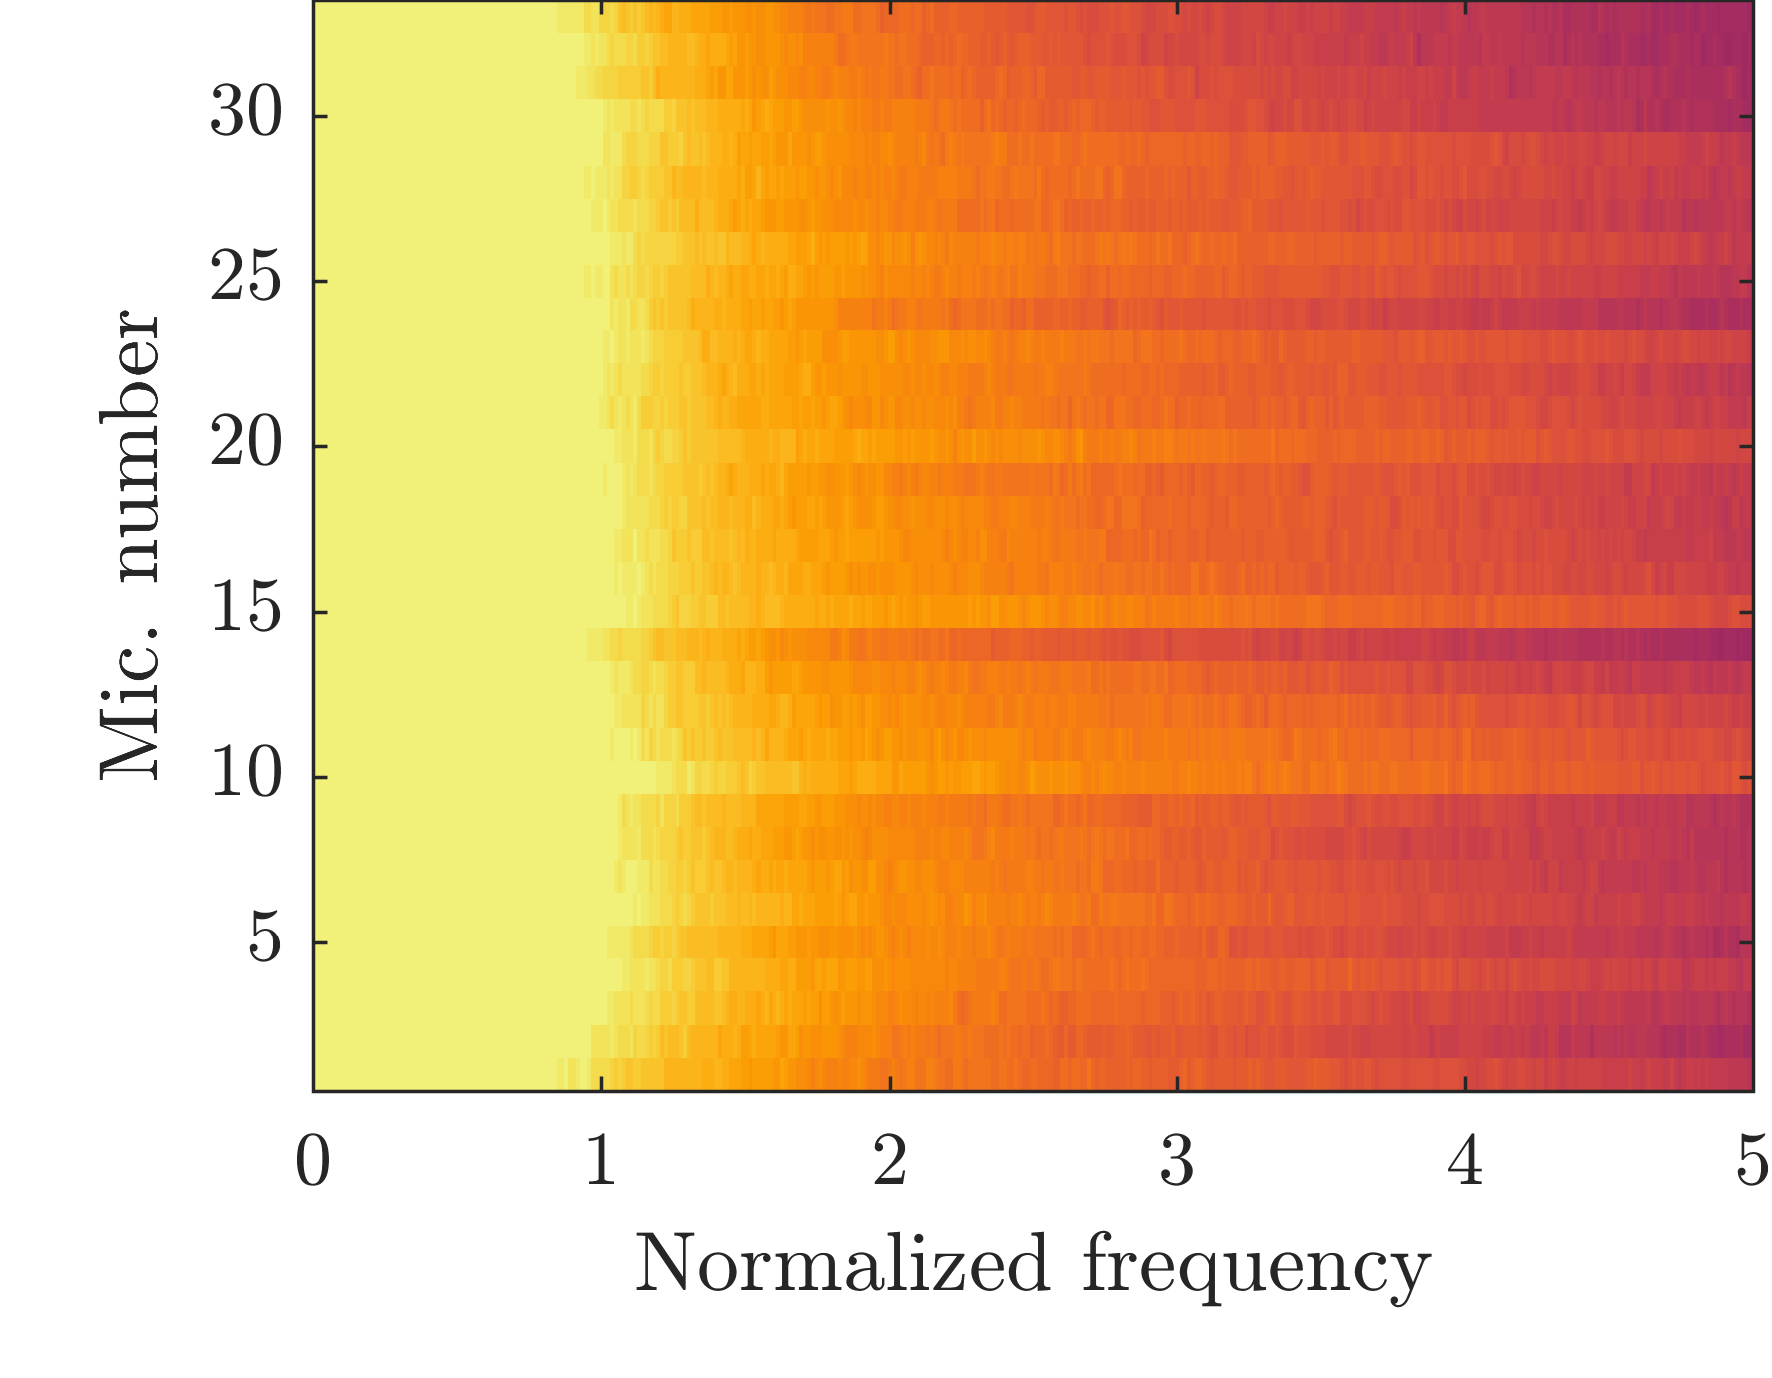
\includegraphics[trim = 2ex 1ex 0 0,clip,width=0.32\textwidth]{./airbus/as_bg.png}} %Background noise (idle engine speed)
		\subfloat[\scriptsize \itshape Débruitage : soustraction du bruit de fond   ]{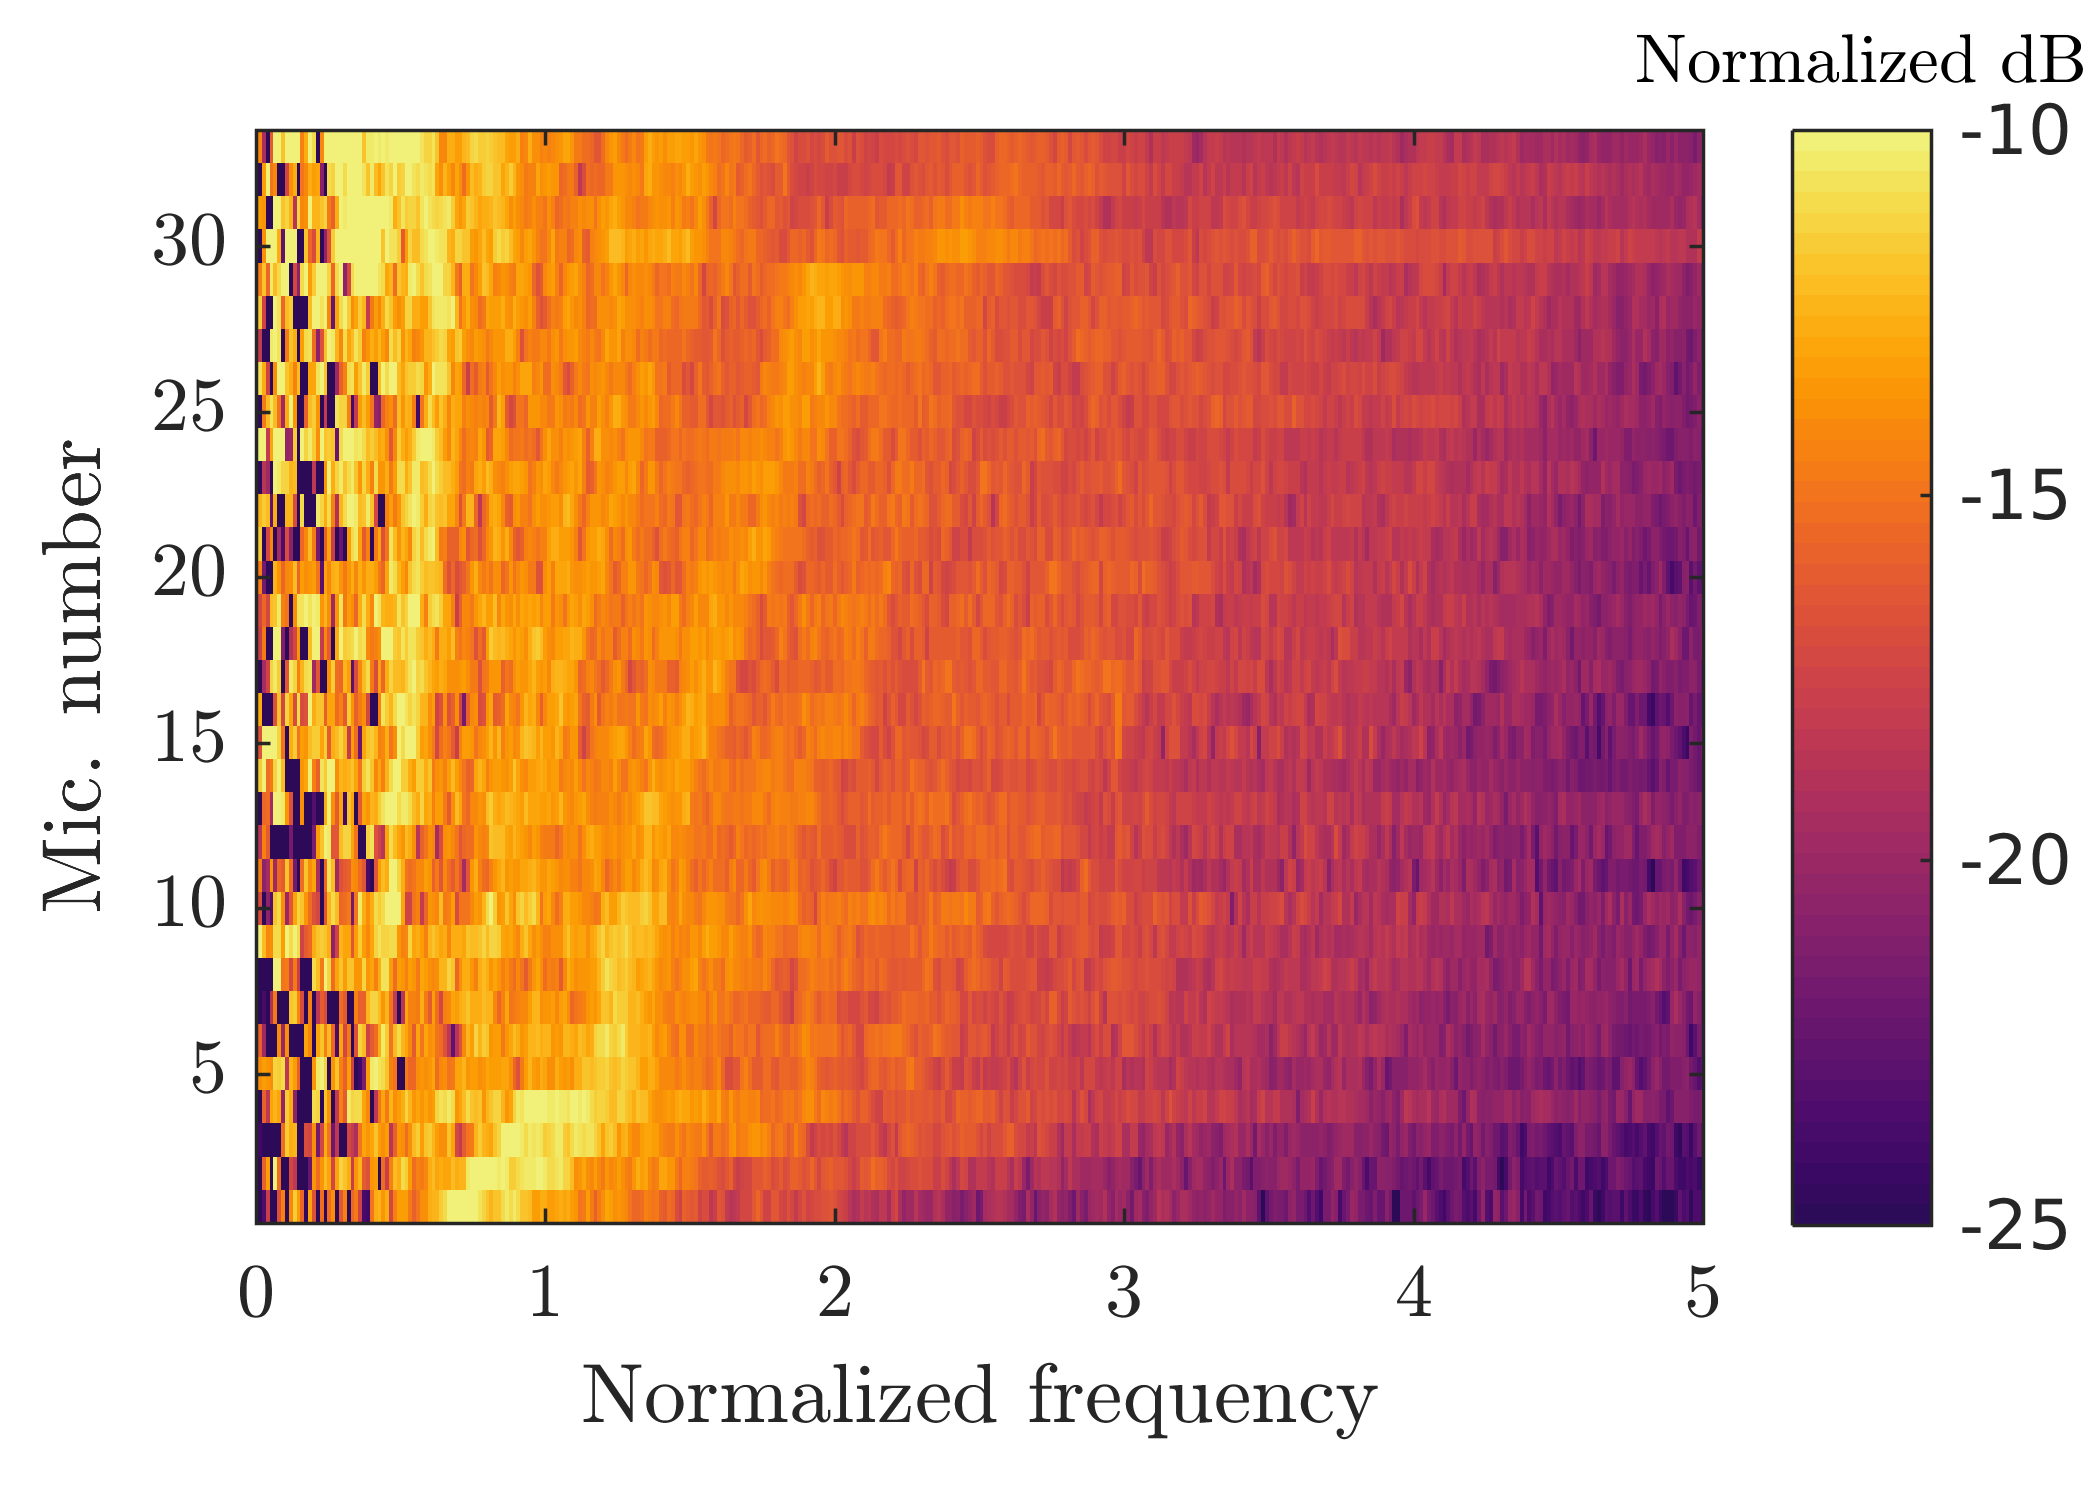
\includegraphics[trim = 1.3ex 1ex 0 0,clip,width=0.385\textwidth]{./airbus/as_bgsub.png}}}\\%Background subtraction
		\hfill \subfloat[\scriptsize  \itshape Débruitage : AFP ]{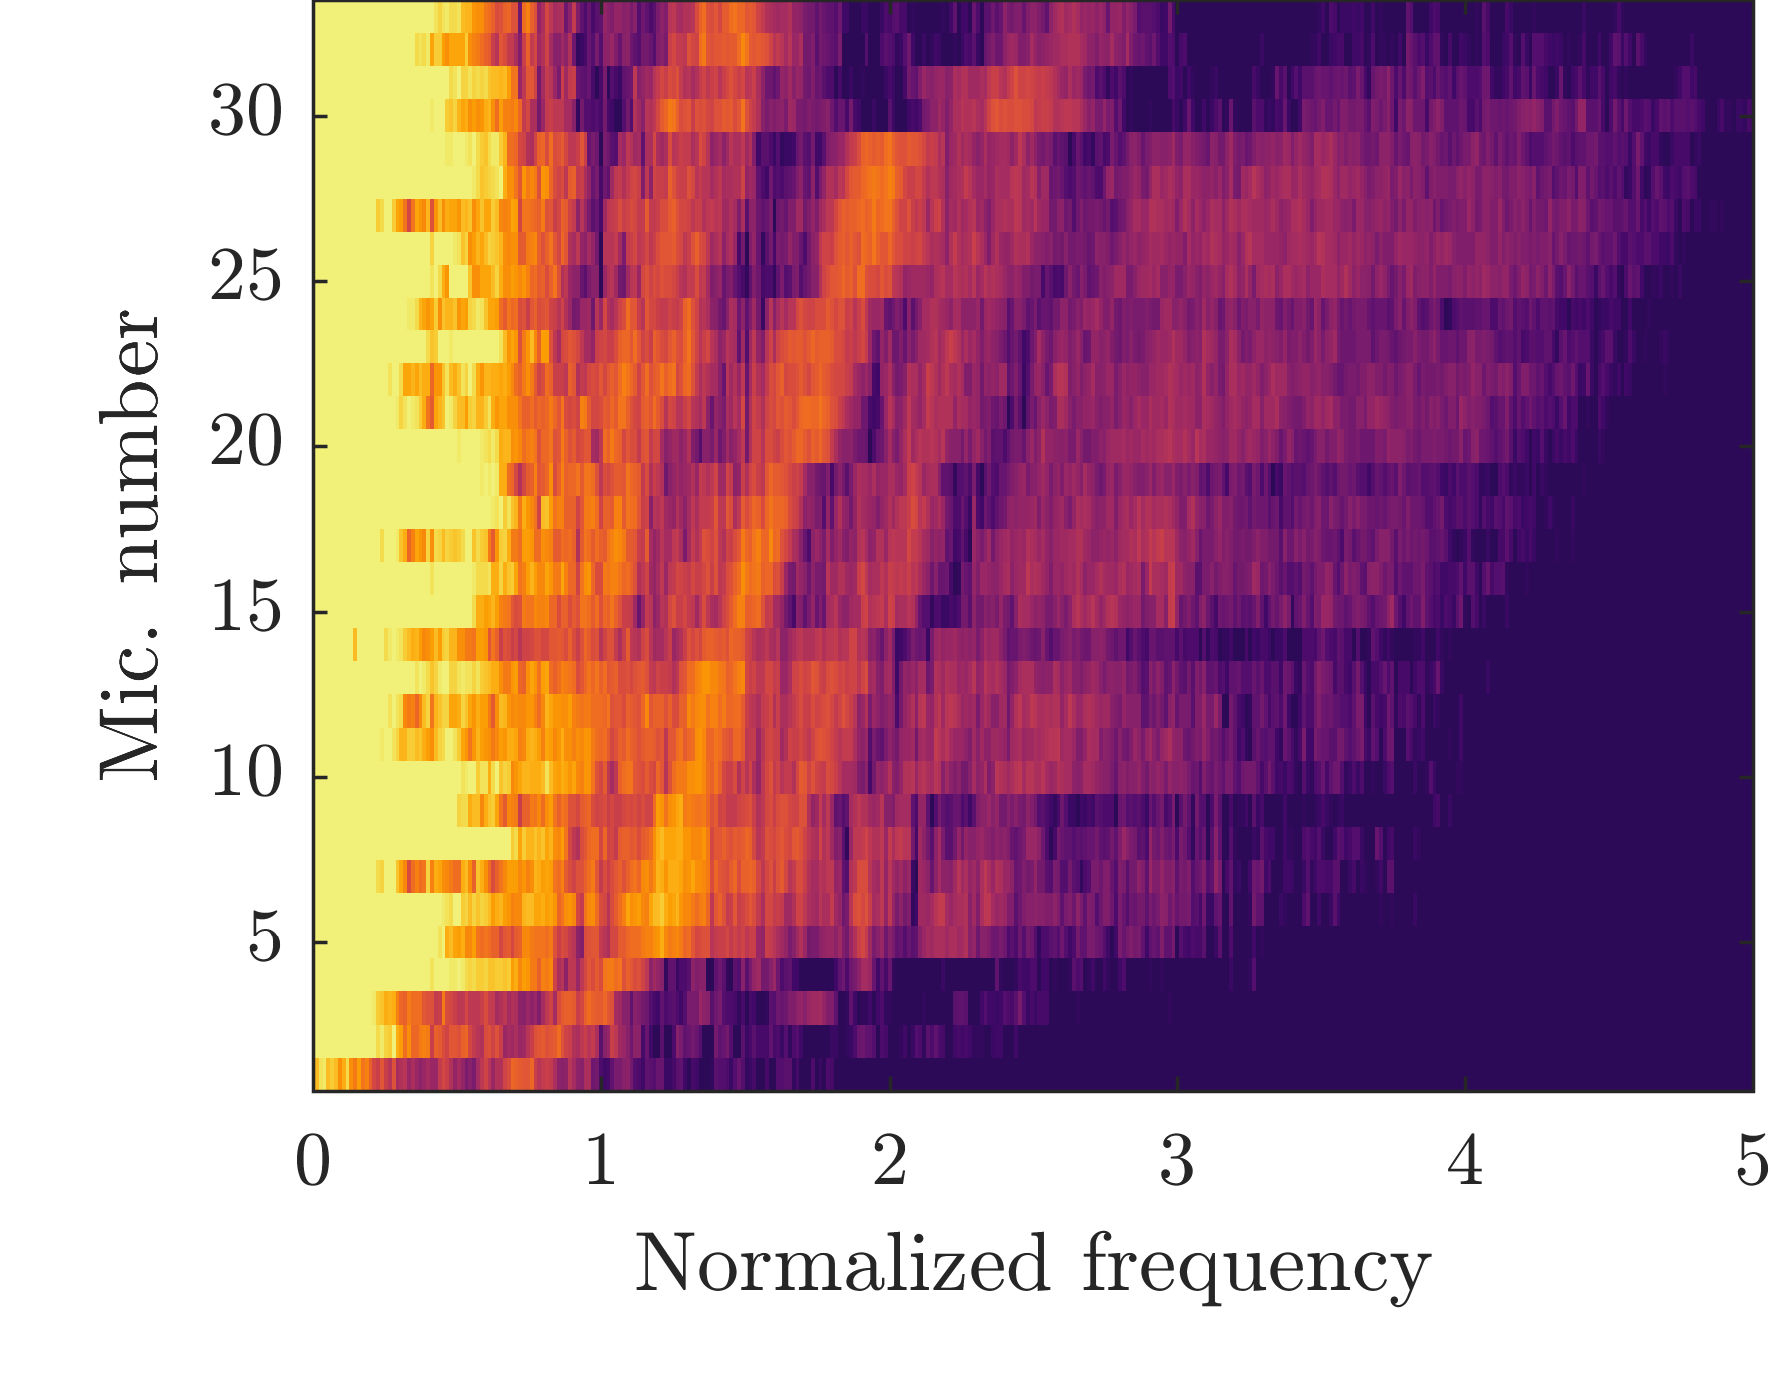
\includegraphics[trim = 2ex 1ex 0 0,clip,width=0.32\textwidth]{./airbus/as_pfa.png}}%PFA denoising
		\subfloat[\scriptsize \itshape Débruitage référencé]{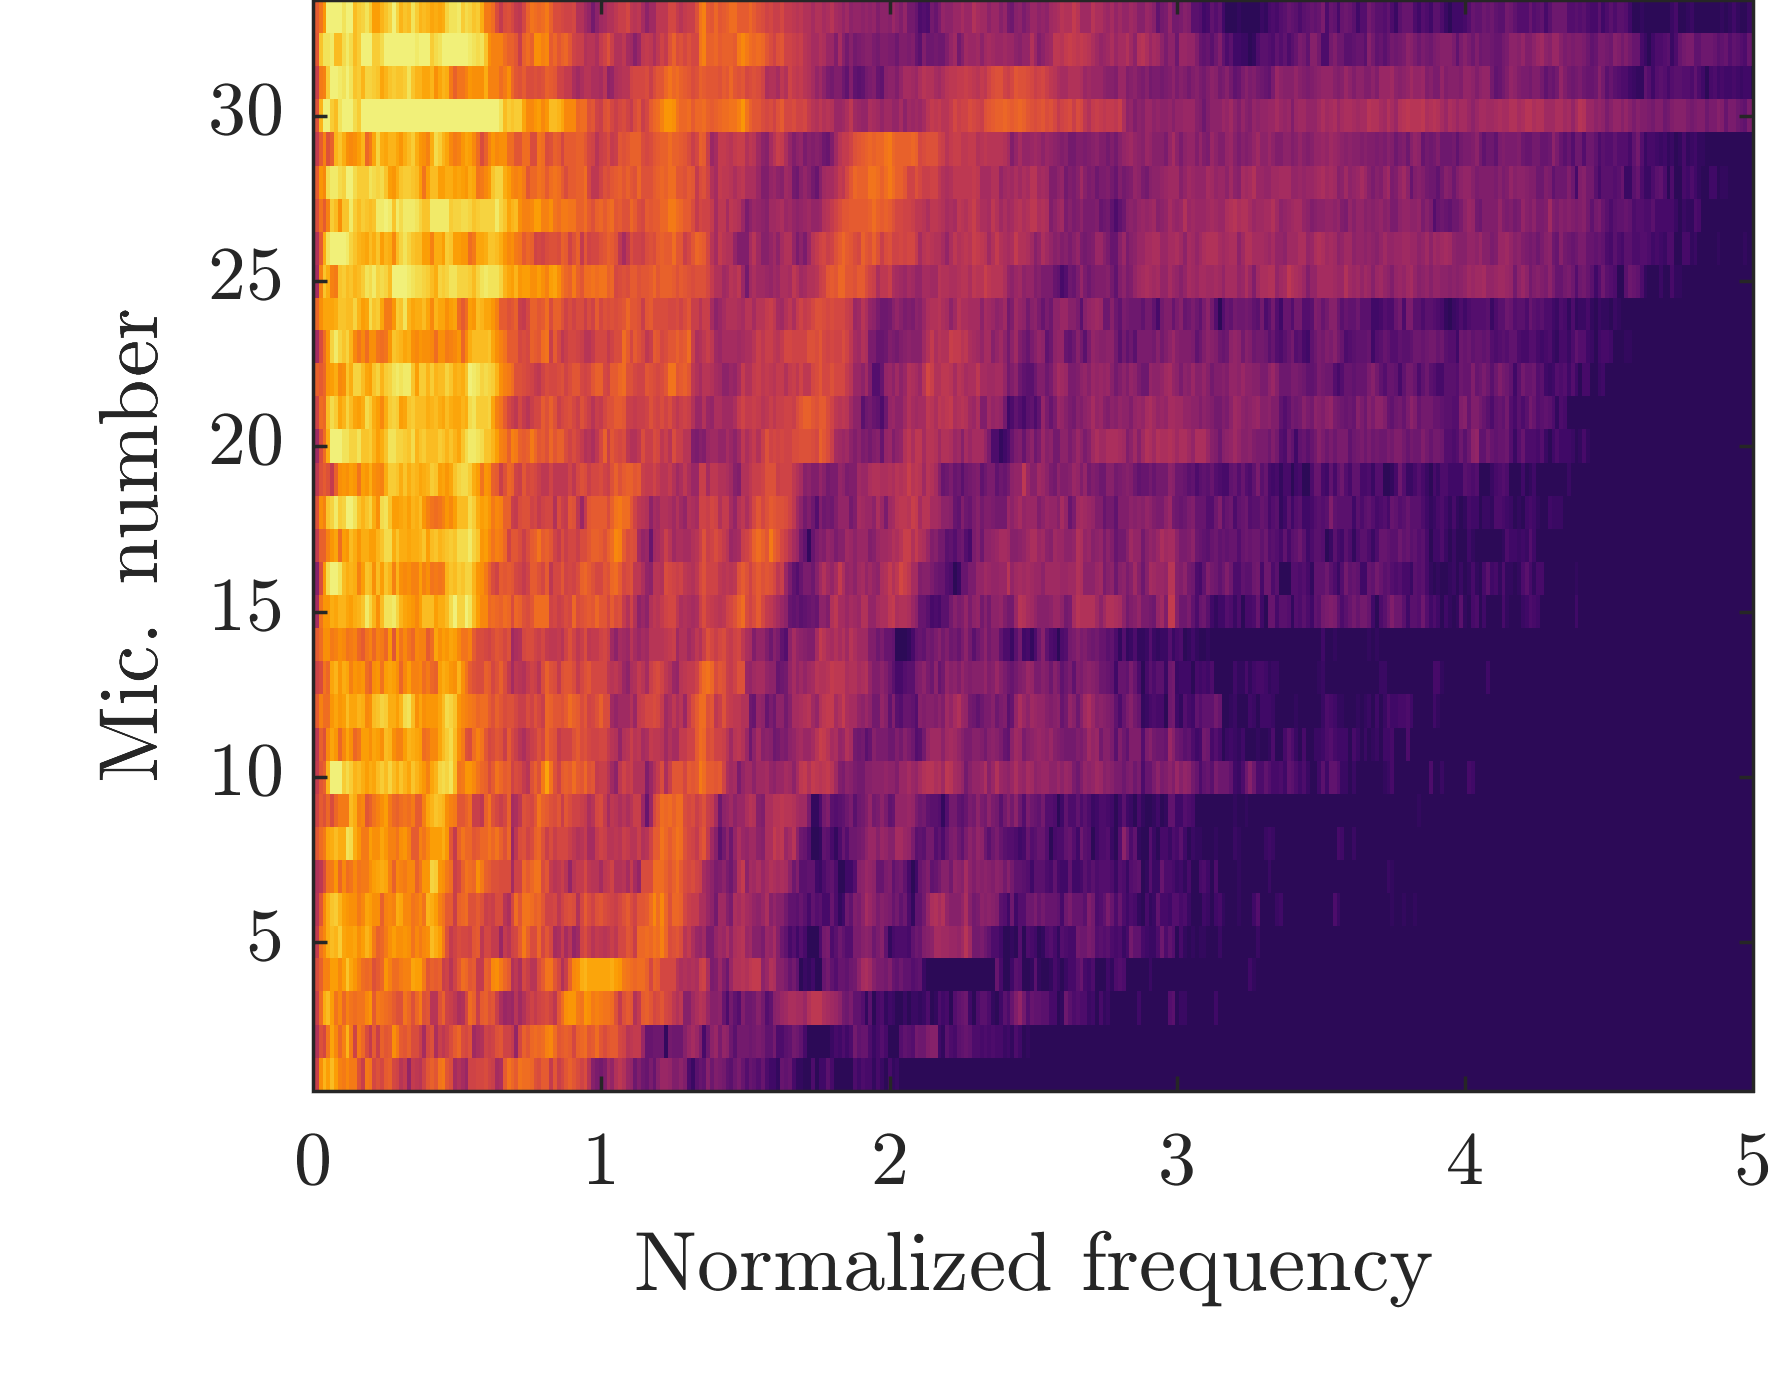
\includegraphics[trim = 2ex 1ex 0 0,clip,width=0.32\textwidth]{./airbus/as_ref.png}}\\% Referenced denoising
	\end{figure}
	}
	\begin{tikzpicture}[remember picture, overlay]
		\node[anchor=south west] (text) at ($(current page.south west)+(1cm,1cm)$) {\begin{minipage}[c][0.28\textwidth][c]{0.35\textwidth}
			\centering \small
			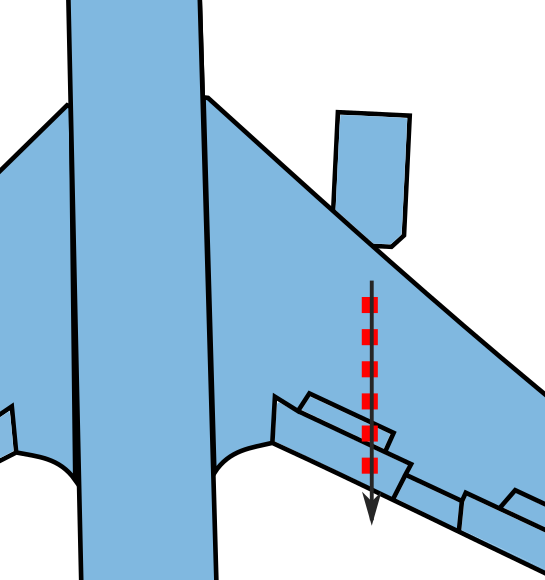
\includegraphics[height=0.5\textwidth]{airbus/jet.png}\\
			\vfill
			\uncover<2->{
				figures d'interférences :\tikzmark{bbsan} \\
				bruit de chocs large bande
			}
			\end{minipage}
		};
		\uncover<2->{
			\node[draw, ellipse,minimum height=2.3cm, minimum width=1.5cm,anchor=west] (interf) at ($(current page.south west)+(5.7,2.5)$) {};
			%\draw[anchor=west] (interf) ellipse (2cm and 1cm);
			\draw[->,>=stealth,line width=1pt] (bbsan) to (interf); 
		}
	\end{tikzpicture}

\end{frame}


\begin{frame}{\insertsectionhead}
	\centering
	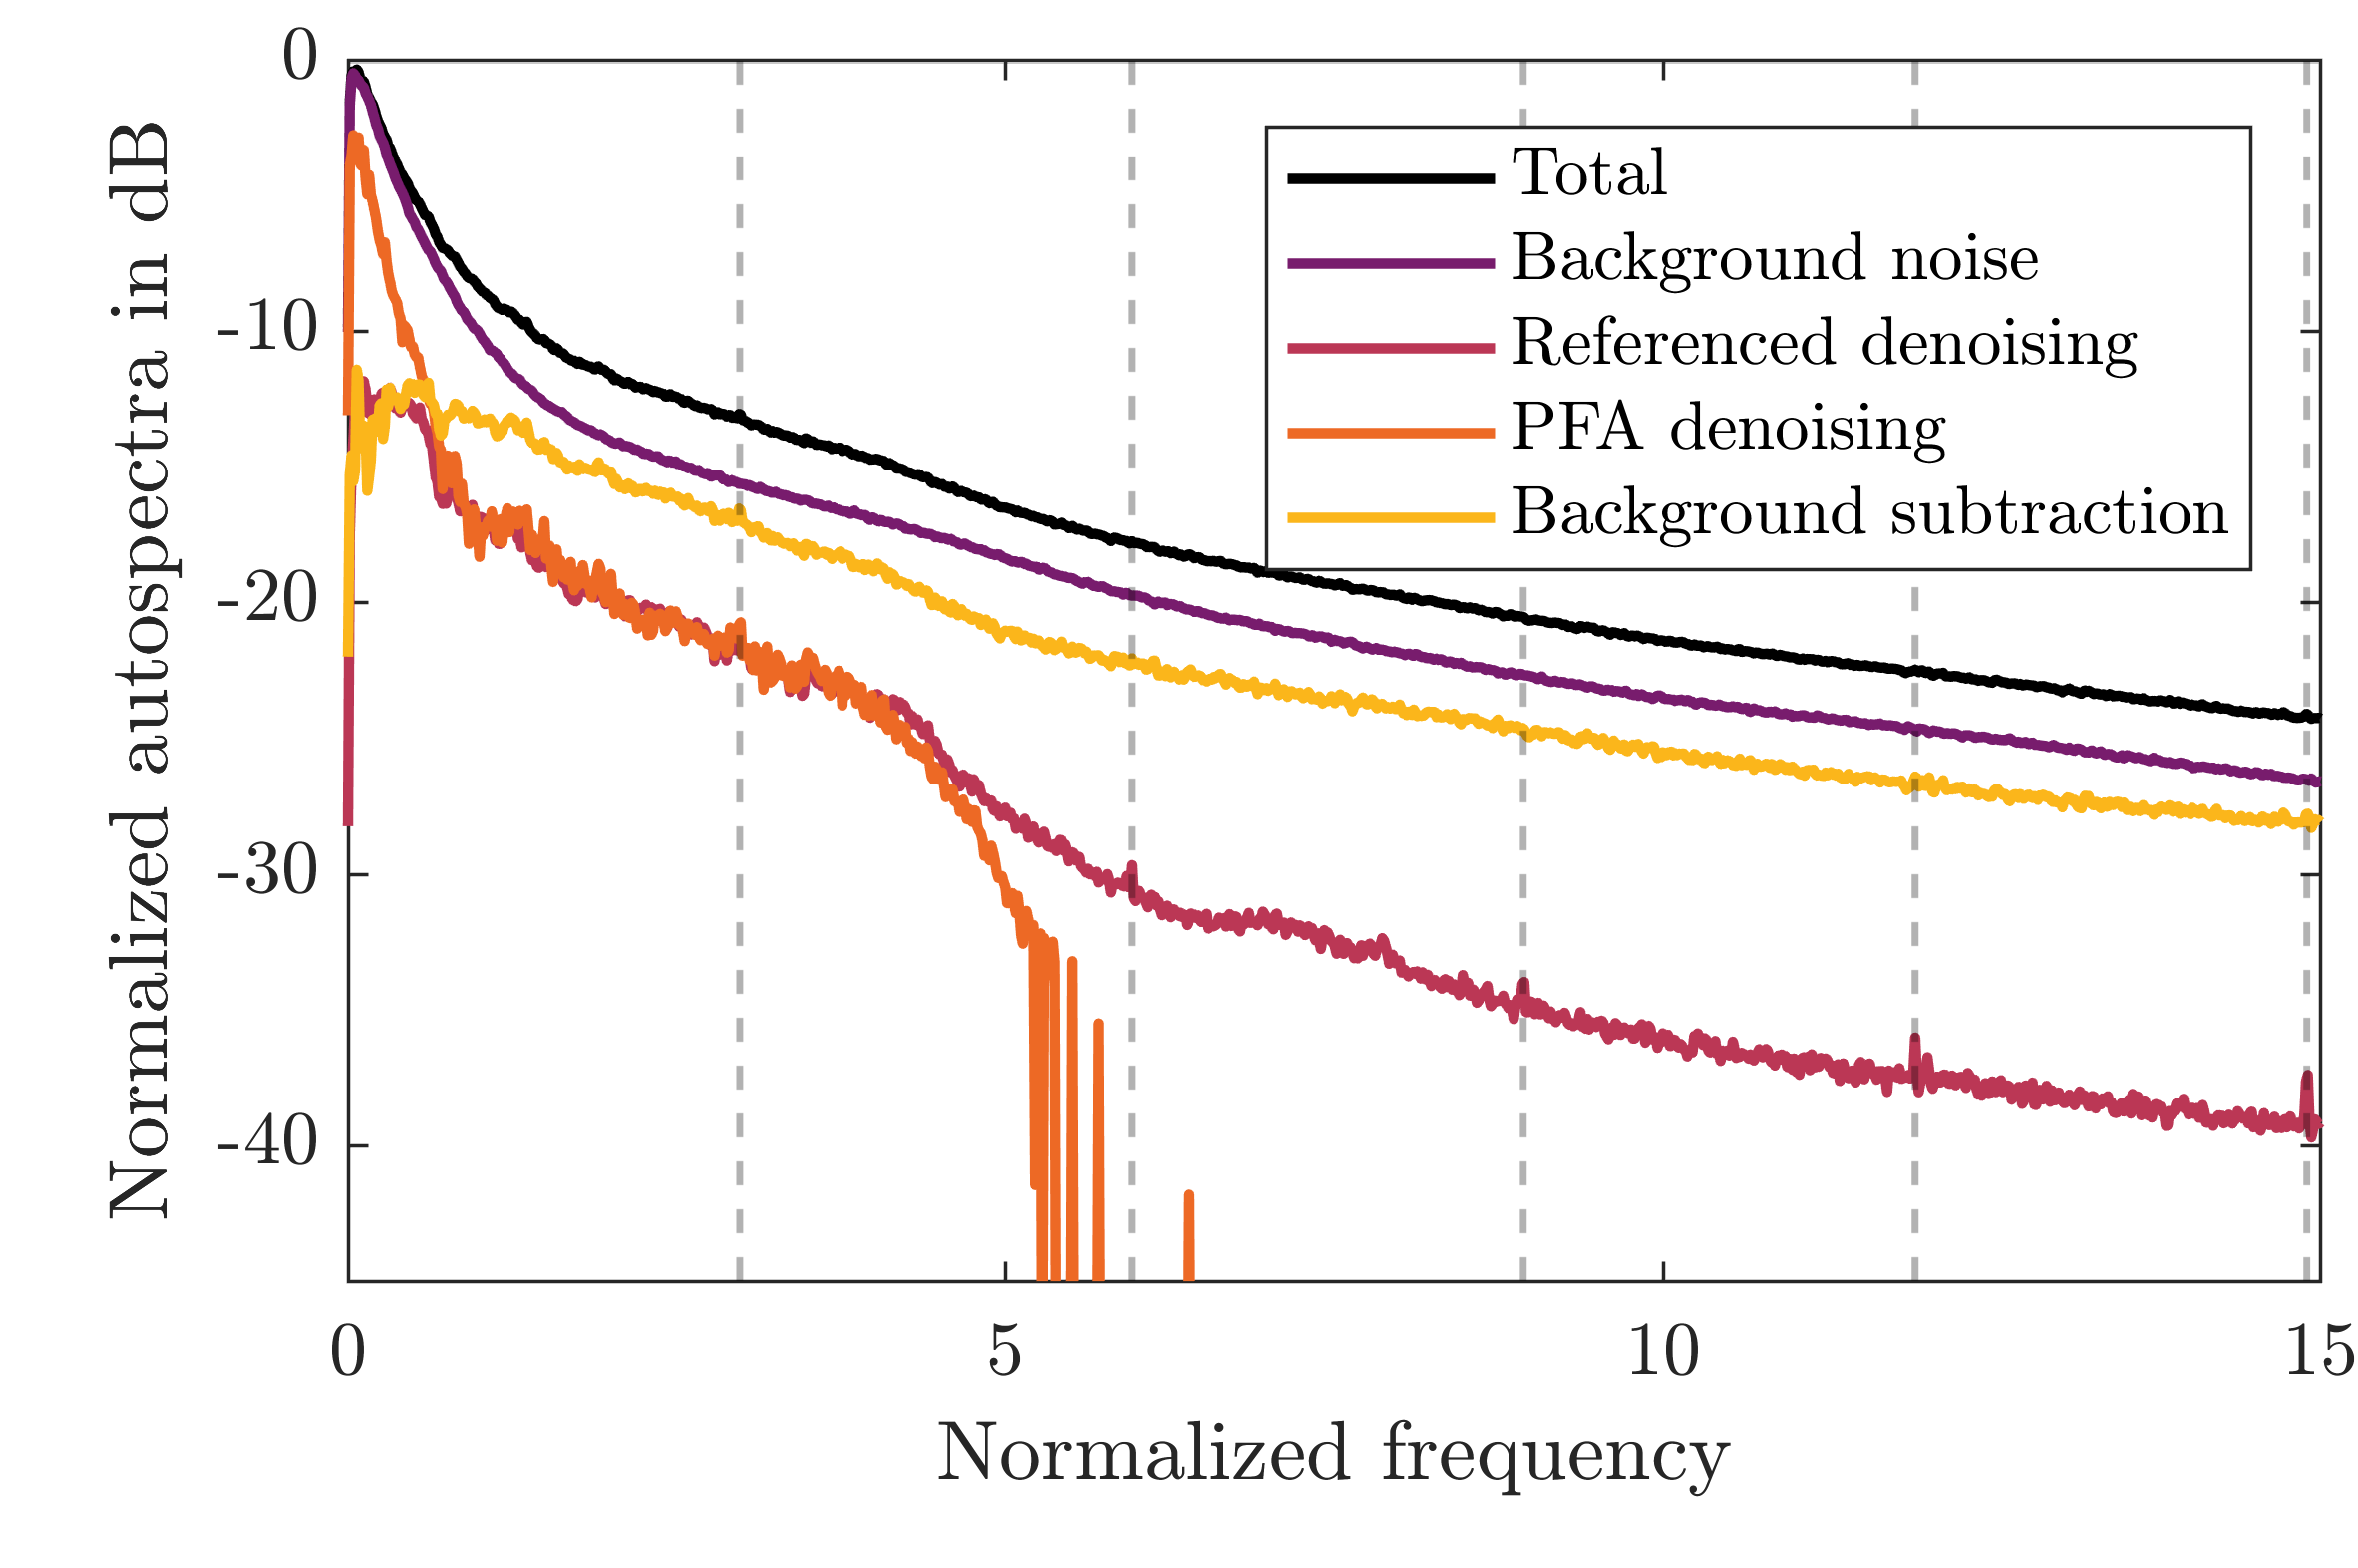
\includegraphics[width=0.7\textwidth]{airbus/mean_as.png}\\
	\vfill
		\begin{itemize}
        		\item Dynamique améliorée de 10-15 dB
        		\item PFA :        \begin{itemize}
       		 	\item Peu de bruit extrait à très basses fréquences $\rightarrow$ bruit corrélé
       		 	\item Pas de signal à moyennes fréquences $\rightarrow$ modèle/priors à adapter
		\end{itemize}
		\item PFA et méthode référencée concordantes en BF
		
	\end{itemize}
\end{frame}

        				%

\begin{frame}[t]{\insertsectionhead~--~Imagerie}
\centering
\textbf{ Méthode inverse}\\
{\small Iterative Reweighted Least Squares, $p=0$ + régularisation baysienne}\\~\\

\begin{minipage}{1.1\textwidth}
	\hspace{-0.65cm}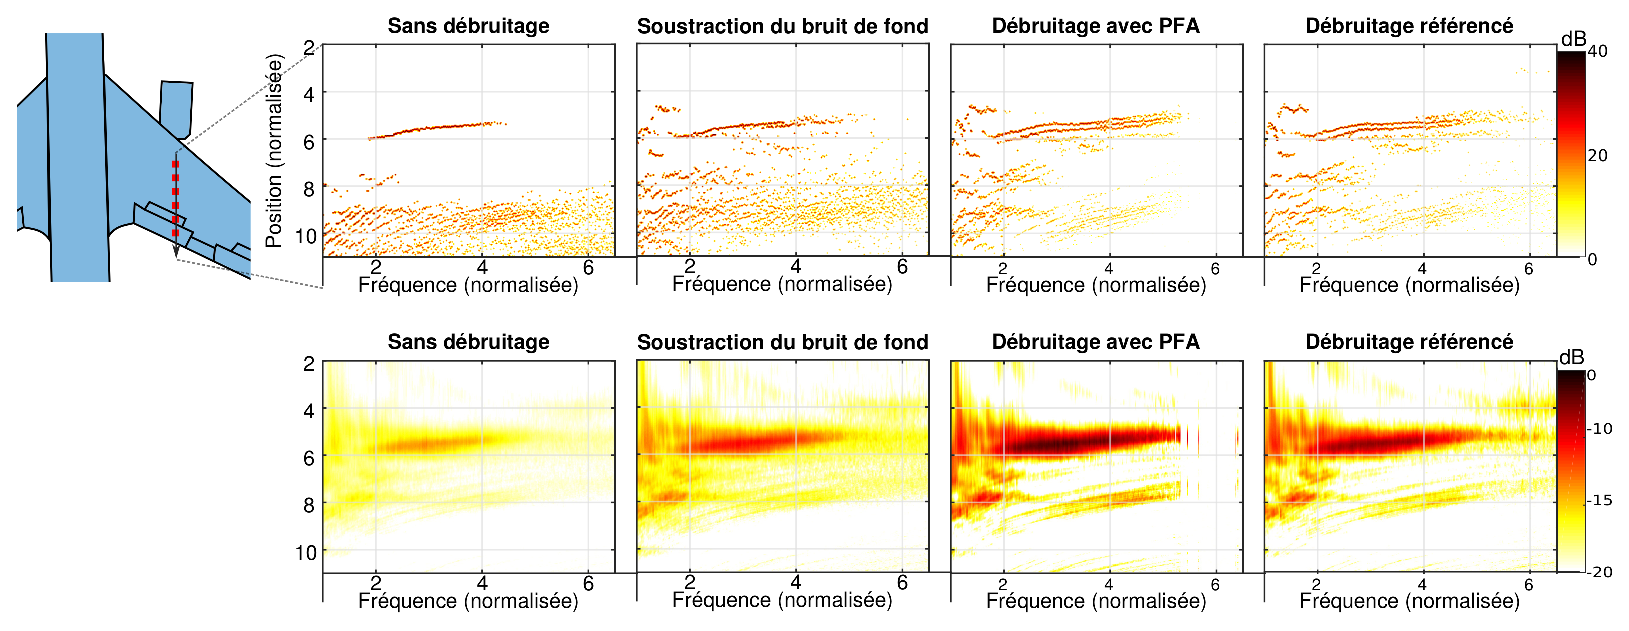
\includegraphics[width=\textwidth]{airbus/imagerie_final.eps}
\end{minipage}~\\~\\~\\
\textbf{Formation de voie}
\end{frame}



\begin{frame}{Conclusions et perspectives}
\begin{itemize}
	\item Débruitage avec différentes hypothèses, mais résultats similaires\\~\\
        \item Amélioration des performances d'imagerie
        \begin{itemize}
       		 \item dynamique
        		\item localisation de sources corrélées
	\end{itemize}~\\
	
	\item Corrections pour l'AFP :
	\begin{itemize}
        		\item augmenter la robustesse de l'échantillonneur
        		\item adapter le modèle statistique (meilleur contrôle de la parcimonie)
        		\item prendre en compte la corrélation du bruit en BF
	\end{itemize}
\end{itemize}

~\\~\\~\\
\vfill

\begin{center}
	\noindent\rule{\textwidth}{0.4pt}
	\scriptsize \itshape{
	This work was performed in the framework of Clean Sky 2 Joint Undertaking, European Union (EU), Horizon 2020, CS2-RIA, ADAPT project, Grant agreement no 754881.}\\
\end{center}

\end{frame}

\begin{frame}{\insertsectionhead~--~Imagerie}
	\centering
	\small
	\begin{equation*}
        		\text{Erreur} = \frac{\|\bm{S}_{aa}^{\text{débruitage}}-\bm{S}_{aa}^{\text{repropagé}}\|_1}{\|\bm{S}_{aa}^{\text{débruitage}}\|_1+\|\bm{S}_{aa}^{\text{repropagé}}\|_1}
	\end{equation*}
	\vfill
	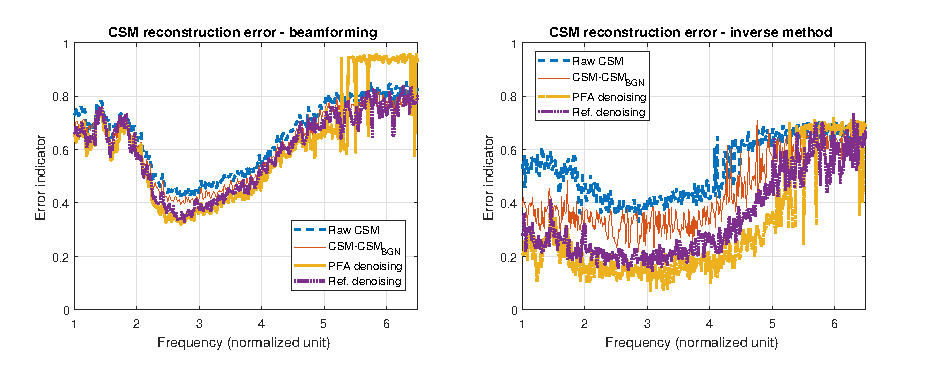
\includegraphics[width=0.9\textwidth]{airbus/erreur.eps}
\end{frame}

\end{document}